% =====================================================================
% CAPITOLO 4 — stesura della candidata, con le correzioni del 9 settembre.
%
% ATTENZIONE: e' ISS-110, questo NON e' `Cap4.tex` del repository.
% ATTENZIONE: il testo consegnato si interrompeva a meta' di §4.10.2. La
% coda e' stata RICOSTRUITA il 9 settembre: parole di chi ricostruisce,
% numeri verificati sui file dei risultati. Il blocco in fondo dice che
% cosa e' stato scritto e su quali file. Va confrontata con l'originale.
% La contraddizione fra 0,630 e la soglia oracolo NON esisteva: sono
% configurazioni e popolazioni di finestre diverse -> ISS-152.
%
% CHE COSA E' CAMBIATO
%
% A. NUMERI CHE NON TORNAVANO CON LE LORO STESSE TABELLE (§4.7.2, §4.7.3)
%    Il testo riportava valori di una tornata precedente. Verificati contro
%    `risultati/addestramento/run_*_tre_classi_DTW_cam1_L22.json`:
%      foresta   testo 0,792 / rec 0,807 / FP 421  ->  tabella e file 0,807 / 0,834 / 501
%      grafo     testo 0,779 +- 0,122               ->  tabella e file 0,699 +- 0,088
%      «recall piu' alta, Transformer 0,939»        ->  la piu' alta e' del grafo, 0,926
%      «meno falsi negativi, Transformer»           ->  il grafo, 104 contro 136
%      GRU-LSTM  testo 0,011 / «oltre cento sogg.»  ->  tabella 0,036 / 57
%    La tabella era giusta, il testo no.
%
% B. UN RISULTATO NUOVO, MISURATO IL 9 SETTEMBRE (§4.7.2)
%    Rieseguendo la foresta con le STESSE dodici grandezze ma con l'ottava e
%    la nona colonna scambiate: F2 da 0,808 a 0,819. Scambiare due colonne
%    adiacenti vale 0,011, cioe' quanto la differenza fra GRU e Random Forest
%    che la §4.7.3 stima richiedere 436 soggetti. E' l'argomento piu' forte
%    del capitolo e non c'era.
%
% C. LE RICHIESTE DEL RELATORE, dalla lettera dell'8 settembre
%    - non «architetture equivalenti» ma «non emerge evidenza sufficiente
%      per attribuire all'architettura un ruolo dominante»
%    - didascalie: dichiarare che le barre sono DEVIAZIONE STANDARD
%    - colonna «Parametri» -> «Parametri addestrabili»
%    - §4.6: non «la geometria e' la causa» ma «i risultati sono coerenti
%      con la geometria della vista come principale spiegazione»
%    - §4.8.3: non «robustezza all'occlusione»; titolo e conclusione rifatti
%    - accanto ai conteggi di FP/FN, riportare anche precision
%
% D. NUMERI CHIARITI O ETICHETTATI
%    - 92,3% (Camera 1) contro 95,9% (entrambe): non e' una contraddizione,
%      ma non era detto. Verificato sui dati.
%    - §4.6: «25 sequenze» -> 39, come dicono la didascalia e i conteggi
%    - §4.8.1: i 4,47 ms sono una misura SUL CALCOLATORE (ISS-137)
%    - §4.3 ha ora l'etichetta `sec:normalizzazione`, che §4.5 citava a vuoto
%
% E. Refusi: «distribuzione non uniforme» -> «non e' uniforme»;
%    «le registrazioni era disgiunte» -> «erano»; due punti fermi mancanti.
%
% VERIFICATO SUI DATI il 2026-09-09: 58.359 fotogrammi, 110 riprese,
% 92,3% di pose valide, etichette 50.264 / 2.771 / 5.324, 11.719 finestre,
% 1.491 positive (12,7%). Tutti esatti. Parametri delle architetture:
% 46147, 24483, 32227, 34499, 12323. Esatti.
% =====================================================================

\chapter{Protocollo di valutazione e risultati sperimentali}
\label{cap:risultati}
\label{cap:protocollo}
\label{cap:sperimentale}

Il valore delle metriche dipende fortemente dalle scelte effettuate durante la valutazione. Infatti, la suddivisione dei soggetti, la normalizzazione delle feature, la gestione dello sbilanciamento e la selezione della soglia decisionale possono alterare sensibilmente il risultato ottenuto, anche mantenendo costanti i dati e il classificatore.
Per questo motivo, in questo capitolo ci concentreremo su due aspetti, ovvero il protocollo utilizzato per la valutazione e i principali risultati sperimentali ottenuti.

Nella prima parte del capitolo vengono stabilite le regole per garantire una valutazione comparabile tra le diverse configurazioni. Discuteremo dello sbilanciamento delle classi, della scelta delle metriche, della separazione dei soggetti fra addestramento e verifica, della normalizzazione delle feature e del criterio utilizzato per trasformare le probabilità del modello in una decisione.

Dopo aver definito il protocollo, analizzeremo i fattori che possono influenzare maggiormente le prestazioni. Considereremo inizialmente l'effetto della geometria di ripresa, per poi passare al confronto tra le varie rappresentazioni del movimento e le architetture di classificazione. Successivamente effettueremo un'analisi di sensibilità, un confronto tra diverse definizioni del compito e, infine, il trasferimento del sistema a un dataset esterno.

\section{Sbilanciamento delle classi e scelta della metrica}

Come discusso nel Capitolo~\ref{cap:contesto}, una caduta è un evento raro rispetto alle normali attività quotidiane; inoltre, un errore che non rileva una caduta non ha lo stesso significato applicativo di un falso allarme. Di conseguenza, la sola accuratezza non è sufficiente per descrivere il comportamento del sistema.

Il sottoinsieme di UP-Fall utilizzato per la valutazione comprende \num{58359} fotogrammi della Camera~1, distribuiti su 110 registrazioni e dieci soggetti. La posa risulta disponibile nel 92,3\% dei fotogrammi di questa vista; considerando entrambe le telecamere la quota sale al 95,9\%, ed è il valore ripreso nella Sezione~\ref{sec:domainshift}. La distribuzione delle annotazioni a livello di fotogramma è riportata in Tabella~\ref{tab:etichette}.

\begin{table}[ht]
\centering
\caption{Distribuzione delle etichette a livello di fotogramma nel sottoinsieme
di UP-Fall utilizzato per la valutazione (Camera~1).}
\label{tab:etichette}
\begin{tabular}{llrr}
\toprule
\textbf{Etichetta} & \textbf{Significato} &
\textbf{Fotogrammi} & \textbf{Quota} \\
\midrule
0 & attività normale / fase precedente & 50.264 & 86,1\% \\
1 & transizione di caduta & 2.771 & 4,7\% \\
2 & stato post-caduta & 5.324 & 9,1\% \\
\bottomrule
\end{tabular}
\end{table}

Dopo la costruzione delle finestre temporali si ottengono complessivamente \num{11719} sequenze, delle quali \num{1491} risultano positive nella configurazione considerata, pari al 12,72\%. Anche all'interno dello stesso dataset la distribuzione fra i soggetti non è uniforme: nei diversi fold di verifica il numero di finestre positive varia infatti da 104 a 171.

Il dataset risulta quindi sbilanciato verso la classe negativa. Questo rende l'accuratezza poco significativa. Un classificatore che assegnasse ogni finestra alla classe negativa otterrebbe infatti un'accuratezza pari a circa l'87,3\%, pur senza riconoscere alcuna caduta.

Per descrivere il comportamento del sistema vengono considerate separatamente precision e recall. Indicando con $TP$ i veri positivi, con $FP$ i falsi positivi e con $FN$ i falsi negativi, la precision è definita come
\[
\mathrm{precision}
=
\frac{TP}{TP+FP},
\]

mentre la recall è
\[
\mathrm{recall}
=
\frac{TP}{TP+FN}.
\]

La recall misura la frazione di cadute effettivamente riconosciute, mentre la precision indica quante delle finestre segnalate come positive corrispondano realmente alla classe di interesse. Nel primo caso una recall ridotta comporta un maggior numero di cadute non rilevate; nel secondo una precision ridotta comporta la generazione di un numero maggiore di falsi allarmi.

Poiché nel contesto considerato si vuole attribuire maggiore importanza alle cadute non rilevate, come misura sintetica viene utilizzato $F_\beta$,
\[
F_\beta =
(1+\beta^2)
\frac{\mathrm{precision}\cdot\mathrm{recall}}
     {\beta^2\,\mathrm{precision}+\mathrm{recall}},
\]

con
\[
\beta=2.
\]

Con questa scelta la recall assume un peso maggiore della precision nella metrica complessiva. Il valore di $\beta$ è stato fissato prima della valutazione dei modelli e non è stato scelto sulla base dei risultati ottenuti.

L'$F_2$ viene comunque utilizzato come indicatore sintetico e non sostituisce l'analisi dei singoli errori. Due configurazioni possono infatti raggiungere valori simili di $F_2$ attraverso combinazioni differenti di precision e recall. Nei confronti successivi vengono quindi considerati anche recall, precision, falsi negativi e falsi positivi, perché variazioni opposte di precision e recall possono produrre valori di $F_2$ simili pur corrispondendo a comportamenti differenti dal punto di vista applicativo.

Lo sbilanciamento viene gestito anche durante l'addestramento. Per ciascun fold vengono assegnati alle classi pesi inversamente proporzionali alla loro frequenza, calcolati esclusivamente sull'insieme di training. In questo modo la classe maggioritaria non domina la funzione di costo, senza dover eliminare una parte consistente delle attività quotidiane disponibili.

Non viene invece utilizzato il sottocampionamento della classe maggioritaria. Con \num{1491} finestre positive su \num{11719}, un riequilibrio completo richiederebbe infatti di eliminare circa tre quarti delle finestre negative, riducendo proprio la varietà delle attività quotidiane che il classificatore deve imparare a non confondere con una caduta.

\section{Partizionamento dei dati e validazione LOSO}
\label{sec:loso}

Un altro problema risiede nel capire come separare i dati utilizzati per l'addestramento da quelli usati per la valutazione. In tale contesto questa scelta è particolarmente importante, poiché ogni soggetto appare in diverse registrazioni, generando così numerose finestre temporali correlate tra loro.

Inizialmente il sottoinsieme utilizzato era composto da cinque soggetti, e la suddivisione veniva eseguita a livello di registrazione. Le riprese risultavano quindi separate fra addestramento e verifica, ma lo stesso soggetto poteva comparire in entrambi gli insiemi: di conseguenza le registrazioni erano disgiunte, le persone no.

Una separazione di questo tipo produce una stima eccessivamente favorevole delle prestazioni. Il modello può infatti utilizzare caratteristiche proprie dei soggetti già osservati durante l'addestramento, come corporatura, proporzioni corporee o modalità individuali di esecuzione del movimento. La valutazione risponde quindi alla domanda di quanto il sistema funzioni su nuove registrazioni delle stesse persone, mentre l'obiettivo del lavoro è valutarne il comportamento su un soggetto non osservato durante l'addestramento. Una differenza analoga fra valutazione su soggetti noti e soggetti non osservati è stata evidenziata anche dallo studio di Scheurer et al.~\cite{scheurer}, che confrontano protocolli subject-dependent e subject-independent su diversi dataset di Human Activity Recognition e mostrano una riduzione consistente delle prestazioni quando la valutazione viene effettuata su soggetti non presenti nel training.

Per evitare questa forma di \emph{subject leakage}, la suddivisione viene effettuata direttamente a livello di soggetto attraverso una validazione \emph{Leave-One-Subject-Out} (LOSO). Con i dieci soggetti considerati vengono quindi implementati dieci fold. In ciascun fold un soggetto viene utilizzato esclusivamente per la verifica finale, un secondo soggetto viene riservato alla validazione e gli otto rimanenti vengono utilizzati per l'addestramento.

Il soggetto di validazione è scelto come quello successivo al soggetto di test secondo un ordinamento circolare. In questo modo la regola è deterministica e i tre insiemi rimangono sempre separati a livello di persona. La composizione dei fold è riportata in Tabella~\ref{tab:fold}.

\begin{table}[ht]
\centering
\caption{Composizione dei dieci fold utilizzati nella validazione LOSO. Per
ogni fold un soggetto è riservato alla verifica, uno alla validazione e gli
otto rimanenti all'addestramento.}
\label{tab:fold}
\begin{tabular}{llrr}
\toprule
\textbf{Soggetto di test} &
\textbf{Validazione} &
\textbf{Finestre di training} &
\textbf{Positive nel test} \\
\midrule
Subject\_01 & Subject\_02 & 9318 & 129 \\
Subject\_02 & Subject\_03 & 9320 & 157 \\
Subject\_03 & Subject\_04 & 9327 & 165 \\
Subject\_04 & Subject\_05 & 9589 & 104 \\
Subject\_05 & Subject\_06 & 9734 & 144 \\
Subject\_06 & Subject\_07 & 9446 & 135 \\
Subject\_07 & Subject\_08 & 9225 & 168 \\
Subject\_08 & Subject\_09 & 9221 & 168 \\
Subject\_09 & Subject\_10 & 9272 & 171 \\
Subject\_10 & Subject\_01 & 9300 & 150 \\
\bottomrule
\end{tabular}
\end{table}

L'utilizzo della LOSO richiede quindi dieci addestramenti indipendenti invece di una singola divisione train/test, ma permette di misurare direttamente la capacità del sistema di operare su una persona non presente nei dati di addestramento. Inoltre evita che finestre molto simili, provenienti dalla stessa registrazione o dallo stesso soggetto, vengano distribuite fra training e test.

Un secondo vantaggio è che il protocollo permette di osservare la variabilità delle prestazioni fra soggetti. Per questo motivo, nei risultati successivi, oltre alla media della metrica viene riportata anche la \textbf{deviazione standard} calcolata sui dieci fold. Tutte le barre di errore delle figure di questo capitolo rappresentano tale quantità, salvo dove diversamente indicato.

Questa dispersione risulta particolarmente importante nel presente dataset. A seconda dell'esperimento, la deviazione standard dell'$F_2$ fra soggetti è generalmente compresa fra circa $0{,}05$ e $0{,}14$, un intervallo confrontabile con molte delle differenze osservate fra configurazioni diverse. Di conseguenza, uno scarto di pochi centesimi nella media non è sufficiente, da solo, per concludere che una configurazione sia effettivamente migliore di un'altra.

Quando due configurazioni vengono valutate sugli stessi soggetti, il confronto viene quindi effettuato fold per fold, mantenendo l'accoppiamento fra i risultati ottenuti sullo stesso individuo. Questo permette di distinguere più correttamente l'effetto della modifica introdotta dalla variabilità dovuta ai soggetti, aspetto che verrà ripreso nel confronto fra rappresentazioni e architetture.

\section{Normalizzazione delle feature}
\label{sec:normalizzazione}

Le feature utilizzate nel presente lavoro descrivono grandezze differenti e assumono quindi scale numeriche anche molto diverse. Nel vettore di ingresso sono presenti, ad esempio, angoli, velocità, rapporti geometrici e grandezze integrali. Se questi valori vengono forniti direttamente al classificatore, le feature caratterizzate da una variabilità numerica maggiore possono assumere un peso eccessivo durante l'addestramento rispetto alle altre.

Nelle prime verifiche questa differenza risultava particolarmente marcata. Il rapporto fra la deviazione standard della feature con scala maggiore e quella con scala minore raggiungeva infatti un valore pari a 646. In queste condizioni il modello tendeva a essere dominato da poche grandezze, mentre il contributo delle feature con valori numericamente più piccoli risultava fortemente ridotto.

Per rendere le diverse grandezze confrontabili è stata quindi applicata una standardizzazione. Indicando con $\mu_j$ e $\sigma_j$ la media e la deviazione standard della feature $j$-esima, il valore trasformato è
\[
z_j =
\frac{x_j-\mu_j}{\sigma_j}.
\]

La stima di $\mu_j$ e $\sigma_j$ viene effettuata separatamente per ciascun fold e utilizzando esclusivamente i soggetti appartenenti all'insieme di training. Gli stessi parametri vengono successivamente applicati ai dati di validation e di test, senza essere ricalcolati. In questo modo il soggetto utilizzato per la verifica non contribuisce alla definizione della trasformazione applicata ai dati.

La normalizzazione viene inoltre stimata sui fotogrammi originali e non sulle finestre temporali. Come descritto nella Sezione~\ref{sec:finestre}, le finestre sono fortemente sovrapposte: con una lunghezza di 22 campioni e un passo pari a 2, lo stesso fotogramma può comparire in più finestre consecutive. Calcolare media e deviazione standard dopo la finestratura significherebbe quindi contare ripetutamente gli stessi campioni, assegnando loro un peso dipendente anche dalla posizione all'interno della registrazione.

Per alcune feature la sola standardizzazione non è sufficiente, perché la distribuzione presenta una forte asimmetria e valori estremi molto distanti dalla maggior parte dei campioni. In questi casi viene applicata preventivamente la trasformazione
\[
x' =
\operatorname{sgn}(x)\log(1+|x|),
\]

che comprime le code della distribuzione mantenendo il segno e l'ordinamento dei valori. La trasformazione viene utilizzata soltanto per le grandezze che soddisfano il criterio previsto nella fase di preprocessing.

Dopo queste operazioni il rapporto fra le scale delle feature si riduce dal valore iniziale di 646 a valori compresi indicativamente fra 1,05 e 1,35. I parametri della trasformazione vengono quindi salvati insieme al modello, perché la stessa normalizzazione deve essere applicata anche durante l'inferenza.

\section{Selezione della soglia decisionale}
\label{sec:soglia}

I classificatori utilizzati nel presente lavoro producono per ogni finestra un punteggio continuo associato alla classe positiva. Per ottenere una decisione binaria è quindi necessario confrontare questo valore con una soglia $\theta$:

\[
\hat{y} =
\begin{cases}
1, & p \geq \theta,\\
0, & p < \theta.
\end{cases}
\]

La scelta di $\theta$ determina il punto di funzionamento del classificatore. Una soglia più bassa aumenta il numero di finestre considerate positive e tende quindi ad aumentare la recall, ma anche i falsi positivi. Una soglia più alta rende invece la decisione più selettiva, riducendo generalmente i falsi allarmi ma aumentando il rischio di perdere alcune cadute.

Nelle prime versioni della pipeline la soglia non era gestita in modo uniforme: parti differenti del codice utilizzavano valori diversi e alcune prove erano state effettuate modificandola manualmente. Una procedura di questo tipo rende difficile confrontare correttamente due configurazioni, perché una parte della differenza osservata può dipendere dal punto di funzionamento scelto e non dal modello stesso.

Una prima soluzione è stata quindi quella di selezionare la soglia sul soggetto di validation di ciascun fold, scegliendo il valore che massimizzava l'$F_2$, e di applicarla successivamente al soggetto di test.

Questa procedura ha però mostrato una forte instabilità. Nei dieci fold le soglie selezionate sono risultate
\[
0{,}01,\;
0{,}02,\;
0{,}22,\;
0{,}43,\;
0{,}71,\;
0{,}75,\;
0{,}90,\;
0{,}94,\;
0{,}95,\;
0{,}99,
\]

con una deviazione standard pari a circa $0{,}37$. Il valore scelto dipende quindi in modo rilevante dal singolo soggetto utilizzato per la validazione e non rappresenta necessariamente un buon punto di funzionamento per il soggetto successivamente utilizzato come test.

Per verificare se una diversa regola potesse fornire una scelta più stabile, sono stati confrontati sei criteri utilizzando le probabilità già prodotte dai dieci fold. Poiché vengono riutilizzati gli stessi punteggi, il confronto non richiede nuovi addestramenti.

\begin{table}[ht]
\centering
\caption{Confronto fra le regole utilizzate per la scelta della soglia
decisionale. Le dispersioni riportate sono deviazioni standard sui dieci fold.}
\label{tab:soglie}
\begin{tabular}{lccc}
\toprule
\textbf{Regola} &
\textbf{$F_2$ medio $\pm$ dev.\ st.} &
\textbf{Recall} &
\textbf{Soglia media $\pm$ dev.\ st.} \\
\midrule
Massimo $F_2$ sul validation
    & 0{,}810 $\pm$ 0{,}117 & 0{,}908 & 0{,}59 $\pm$ 0{,}37 \\
Massimo $F_1$
    & 0{,}790 $\pm$ 0{,}120 & 0{,}851 & 0{,}70 $\pm$ 0{,}34 \\
Indice di Youden
    & 0{,}808 $\pm$ 0{,}117 & 0{,}910 & 0{,}59 $\pm$ 0{,}37 \\
Prevalenza
    & 0{,}787 $\pm$ 0{,}116 & 0{,}858 & 0{,}68 $\pm$ 0{,}35 \\
Prevalenza maggiorata
    & 0{,}823 $\pm$ 0{,}136 & 0{,}972 & 0{,}43 $\pm$ 0{,}31 \\
Soglia fissa $\theta=0{,}50$
    & 0{,}851 $\pm$ 0{,}078 & 0{,}926 & 0{,}50 $\pm$ 0{,}00 \\
\bottomrule
\end{tabular}
\end{table}

La soglia fissa a $0{,}50$ presenta, in questo confronto, il valore medio di $F_2$ più elevato e la dispersione più bassa. Le regole che stimano la soglia sul singolo soggetto di validation introducono invece una variabilità elevata, che in questo caso risulta maggiore del beneficio ottenuto adattando il punto di decisione al soggetto.

Questo risultato deve tuttavia essere interpretato con cautela. Le sei regole sono state confrontate utilizzando i risultati dei fold di test e non sarebbe quindi corretto concludere, a posteriori, che $0{,}50$ sia la soglia ottimale del problema. L'esperimento mostra invece che la stima della soglia a partire da un solo soggetto di validation è poco stabile.

Per i confronti successivi viene quindi adottata una soglia fissa
\[
\theta = 0{,}50,
\]

uguale per tutti i fold e per tutte le configurazioni considerate. In questo modo la soglia non introduce un ulteriore parametro dipendente dal soggetto e le differenze osservate possono essere attribuite più direttamente alla configurazione che si sta confrontando.

\section{Effetto congiunto delle correzioni introdotte nel protocollo}
\label{sec:baseline}

Le modifiche descritte nelle sezioni precedenti non riguardano l'architettura del classificatore, ma il modo in cui i dati vengono preparati e valutati. È quindi utile verificare quale effetto producano mantenendo invariati, per quanto possibile, i dati e il modello utilizzato.

Nella configurazione iniziale il classificatore non riconosceva alcun esempio positivo, producendo un valore di $F_1$ pari a zero. L'analisi della pipeline ha evidenziato tre problemi principali: l'assenza di una normalizzazione coerente delle feature, la separazione dei dati per registrazione anziché per soggetto e l'utilizzo dello stesso insieme sia per alcune scelte di modello sia per la verifica finale.

La configurazione corretta introduce invece la normalizzazione descritta nella Sezione~\ref{sec:normalizzazione}, la separazione dei soggetti mediante LOSO e un insieme di validation distinto dal soggetto utilizzato per il test.

\begin{table}[ht]
\centering
\caption{Effetto congiunto delle principali correzioni introdotte nel
protocollo di valutazione.}
\label{tab:correzioni}
\begin{tabular}{lcc}
\toprule
 & \textbf{Configurazione iniziale} &
   \textbf{Configurazione corretta} \\
\midrule
$F_1$ & 0,000 & 0,234 \\
Veri positivi & 0 & 144 \\
Rapporto massimo fra le scale & 646$\times$ & 1,05--1,35$\times$ \\
Soggetti condivisi fra training e test & 5 su 5 & 0 \\
\bottomrule
\end{tabular}
\end{table}

Il passaggio da zero a 144 veri positivi mostra che il fallimento iniziale non era dovuto alla sola capacità del classificatore. Allo stesso tempo, il valore di $F_1=0{,}234$ rimane troppo basso per poter considerare risolto il problema. Le correzioni permettono quindi di ottenere una valutazione significativa, ma non spiegano ancora quali siano i fattori che limitano maggiormente le prestazioni.

Una volta fissato un protocollo coerente, è possibile analizzare separatamente questi fattori. Il primo riguarda la geometria con cui il movimento viene osservato.

\section{Effetto della geometria di ripresa}
\label{sec:viewpoint}

Il primo fattore analizzato è il punto di vista della telecamera. UP-Fall permette di studiarlo in una condizione particolarmente utile, perché lo stesso evento viene acquisito contemporaneamente da due camere: una vista laterale, posta approssimativamente all'altezza del busto, e una vista frontale rialzata. Il soggetto e il movimento sono quindi gli stessi e cambia principalmente la geometria di osservazione.

I risultati di questa sezione sono stati rimisurati su tutti e dieci i soggetti e sul dataset riestratto. Una versione precedente, a cinque soggetti, dava valori diversi: la direzione dell'effetto non è cambiata, la sua ampiezza sì.

Una delle grandezze maggiormente associate alla dinamica di una caduta è la variazione dell'inclinazione del tronco. La sua osservabilità dipende però dal piano di proiezione. Una rotazione che appare evidente in una vista laterale può risultare molto più ridotta quando la persona viene osservata frontalmente e dall'alto.

Delle cinquanta riprese di caduta disponibili, undici sono state escluse per la ragione data più sotto; la Tabella~\ref{tab:escursione} riporta quindi l'escursione dell'angolo del tronco misurata sulle trentanove rimanenti.

\begin{table}[ht]
\centering
\caption{Escursione dell'angolo del tronco nelle due viste considerate. Dieci
soggetti; sono escluse le undici riprese in cui lo stimatore di posa cambia
persona, e ne restano trentanove.}
\label{tab:escursione}
\begin{tabular}{lcc}
\toprule
 & \textbf{Camera 1} & \textbf{Camera 2} \\
 & \textbf{laterale} & \textbf{frontale rialzata} \\
\midrule
Escursione media & 74,0$^\circ$ & 33,2$^\circ$ \\
Sequenze con escursione $>60^\circ$ & 30/39 & 8/39 \\
\bottomrule
\end{tabular}
\end{table}

L'escursione media osservata dalla Camera~1 è quindi quasi doppia rispetto a quella della Camera~2. Il rapporto fra le medie non descrive però completamente il fenomeno, perché la variabilità fra le singole cadute rimane elevata. Le deviazioni standard sono infatti pari rispettivamente a $24{,}2^\circ$ e $23{,}5^\circ$, mentre il rapporto fra le due escursioni varia, nelle singole sequenze, da 0,98 a 7,37, con mediana 2,79. In un solo caso la vista rialzata osserva un'escursione pari a quella laterale.

La Figura~\ref{fig:viewpoint_dist} mostra questo confronto mantenendo l'accoppiamento fra le due riprese dello stesso evento.

\begin{figure}[ht]
\centering
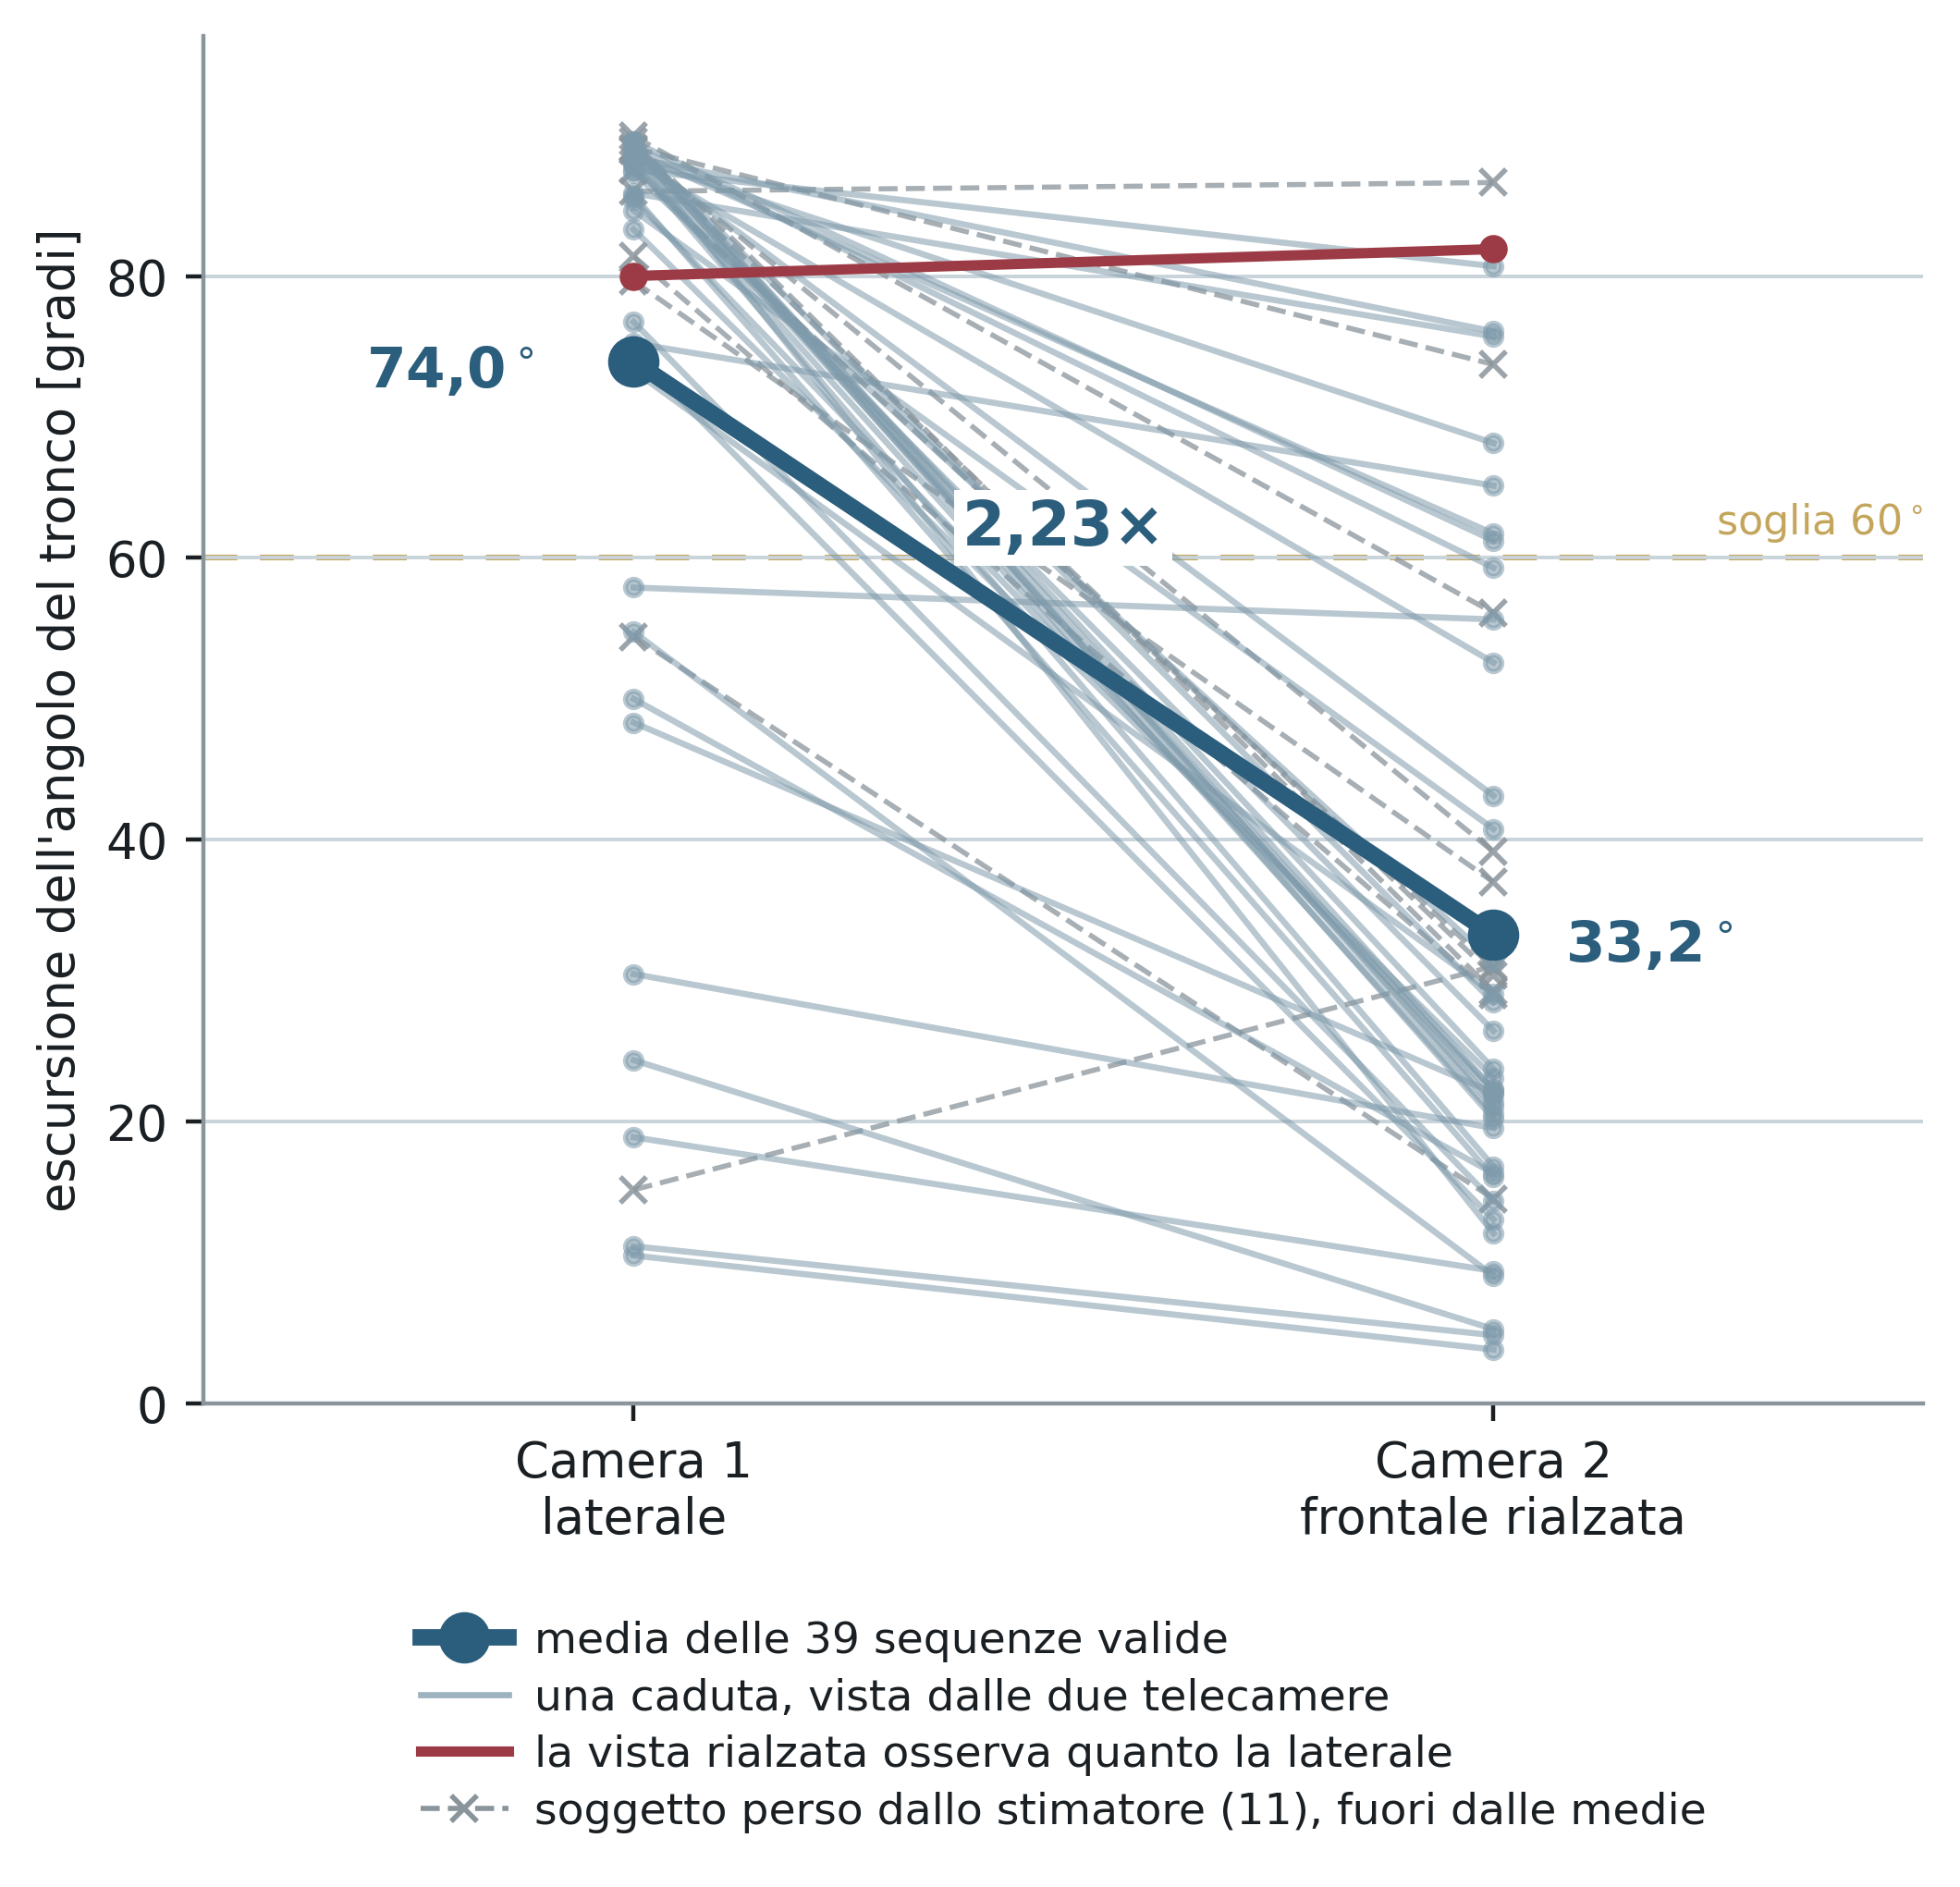
\includegraphics[width=.78\textwidth]{figure/fig_viewpoint_dist.png}
\caption{Escursione dell'angolo del tronco nelle due viste per le trentanove
sequenze in cui entrambe le viste seguono il soggetto.}
\label{fig:viewpoint_dist}
\end{figure}

Nel rifare questa misura sono emersi due difetti del codice che la produceva. Il primo: un unico stimatore di posa veniva riusato per tutte le riprese in successione, e poiché MediaPipe Pose mantiene stato fra fotogrammi, l'ultima immagine di una ripresa condizionava la prima della successiva --- su una sequenza lo scarto arriva a $68^\circ$. Il secondo, più rilevante: su Camera~2 lo stimatore perde chi cade e si aggancia a una persona rimasta in piedi, in 11 riprese su 50, contro 0 su 50 di Camera~1. Le undici riprese contaminate sono escluse dalle medie.

La differenza geometrica si riflette anche sulle prestazioni del classificatore. Nella stessa configurazione sperimentale, utilizzando la sola vista laterale si ottiene un $F_2$ pari a circa 0,822, mentre il trasferimento di un modello addestrato sulla Camera~1 verso la Camera~2 porta il valore a 0,488.

\begin{table}[ht]
\centering
\caption{Trasferimento fra le due viste. LOSO a dieci soggetti, foresta
casuale, rappresentazione A3, soglia $0{,}50$ dichiarata a priori. Le
dispersioni sono deviazioni standard sui dieci fold. La quarta riga non
riguarda il trasferimento e serve al confronto discusso più sotto.}
\label{tab:viste}
\begin{tabular}{lccc}
\toprule
\textbf{Training} & \textbf{Test} & \textbf{$F_2$} &
\textbf{Falsi positivi} \\
\midrule
Camera 1 & Camera 1 & $0{,}822 \pm 0{,}099$ & 722 \\
Camera 1 & Camera 2 & $0{,}488 \pm 0{,}119$ & 3252 \\
Camera 1 + Camera 2 & Camera 2 & $0{,}731 \pm 0{,}188$ & 751 \\
\midrule
Camera 2 & Camera 2 & $0{,}753 \pm 0{,}179$ & 1067 \\
\bottomrule
\end{tabular}
\end{table}

Il solo cambio di inquadratura produce quindi una riduzione di circa 0,334 di $F_2$, circa tre volte la dispersione fra soggetti.

Il risultato migliora quando entrambe le viste vengono utilizzate durante l'addestramento. Sul test effettuato con Camera~2 l'$F_2$ passa infatti da 0,488 a 0,731 e i falsi allarmi diminuiscono da 3252 a 751. Anche recall e precision migliorano contemporaneamente, passando rispettivamente da 0,670 a 0,762 e da 0,316 a 0,713: il guadagno non deriva quindi da un semplice spostamento del punto di funzionamento fra i due tipi di errore.

Questo risultato indica che la variabilità del punto di vista può essere appresa almeno in parte se viene rappresentata nei dati di training. Rimane comunque un divario rispetto alla condizione in cui addestramento e test utilizzano la vista laterale.

Va precisato in che senso la geometria intervenga. Questi risultati \emph{non dimostrano} che la geometria della vista sia la causa del degrado osservato: mostrano che essa ne è una spiegazione coerente con tutte le misure disponibili, e che la spiegazione alternativa più immediata --- la perdita di tracciamento --- non basta a rendere conto del fenomeno, dal momento che il divario permane anche escludendo le undici riprese in cui essa si verifica. La geometria di ripresa risulta comunque una delle variabili con maggiore effetto sul sistema, e l'aspetto verrà ripreso nel Capitolo~\ref{cap:campo}, dove il posizionamento della telecamera diventa parte del protocollo di installazione.

\section{Confronto fra rappresentazioni e architetture}

Una volta evidenziato l'effetto della geometria di ripresa, è possibile confrontare due scelte interne alla pipeline: la rappresentazione fornita al classificatore e l'architettura utilizzata per elaborarla.

In entrambi i casi il confronto viene effettuato mantenendo invariato il resto del protocollo. Questo è necessario perché gli scarti osservati sono molto più piccoli di quello prodotto dal cambio di telecamera e spesso dello stesso ordine della variabilità fra soggetti.

\subsection{Confronto fra rappresentazioni}
\label{sec:featureset}

Le tre rappresentazioni geometriche A1, A2 e A3 descritte nel Capitolo~\ref{cap:metodologia} sono state inizialmente confrontate nella configurazione sperimentale a cinque soggetti.

\begin{table}[ht]
\centering
\caption{Confronto preliminare fra le tre rappresentazioni geometriche.
Esperimento condotto su cinque soggetti; le dispersioni sono deviazioni
standard fra i fold.}
\label{tab:rappresentazioni5}
\begin{tabular}{lcc}
\toprule
\textbf{Rappresentazione} & \textbf{$F_2$} & \textbf{Recall} \\
\midrule
A1 --- piano immagine & $0{,}834 \pm 0{,}121$ & -- \\
A2 --- world landmarks 3D & $0{,}867 \pm 0{,}099$ & -- \\
A3 --- riferimento corporeo & $0{,}857 \pm 0{,}088$ & 0,929 \\
\bottomrule
\end{tabular}
\end{table}

Il valore medio più alto è ottenuto da A2, ma la differenza complessiva fra la migliore e la peggiore rappresentazione è pari a 0,033, mentre le deviazioni standard variano fra 0,088 e 0,121. I risultati non permettono quindi di stabilire una superiorità fra le tre rappresentazioni.

Questo confronto presenta inoltre un limite emerso successivamente durante l'analisi del motore geometrico. Due delle grandezze utilizzate in A2 erano state definite rispetto alla traslazione del bacino nei \emph{world landmarks}. Poiché MediaPipe utilizza proprio il bacino come origine del sistema di riferimento, queste grandezze risultavano quasi degeneri. Le due feature sono state successivamente rimosse o ridefinite, come descritto nel Capitolo~\ref{cap:metodologia}. Il risultato della Tabella~\ref{tab:rappresentazioni5} deve quindi essere letto come una verifica preliminare e non come una classifica definitiva.

Dopo la correzione è stato effettuato un secondo confronto su dieci soggetti, questa volta concentrato sull'effetto delle diverse configurazioni di feature utilizzate nella pipeline finale.

\begin{table}[ht]
\centering
\caption{Confronto fra tre configurazioni di feature su dieci soggetti; le
dispersioni sono deviazioni standard fra i dieci fold.}
\label{tab:rappresentazioni10}
\begin{tabular}{lc}
\toprule
\textbf{Configurazione} & \textbf{$F_2$} \\
\midrule
A3 senza grandezze integrali & $0{,}874 \pm 0{,}080$ \\
A3 con grandezze integrali & $0{,}858 \pm 0{,}075$ \\
Sottoinsieme selezionato tramite DTW & $0{,}857 \pm 0{,}078$ \\
\bottomrule
\end{tabular}
\end{table}

Anche in questo caso le differenze sono molto ridotte. Fra il valore maggiore e quello minore vi sono soltanto 0,017 punti di $F_2$, contro una dispersione fra soggetti di circa 0,08.

Il risultato non indica quindi che le grandezze integrali o la selezione tramite DTW peggiorino il classificatore. Indica piuttosto che, all'interno di UP-Fall e con questa numerosità, le tre configurazioni non sono distinguibili sulla base della sola prestazione media. L'utilità delle rappresentazioni temporali verrà valutata nuovamente nel trasferimento a un dataset esterno, dove le differenze risultano più evidenti.

\subsection{Confronto fra architetture}
\label{sec:architetture}

Il secondo confronto riguarda l'architettura del classificatore. L'ipotesi iniziale del progetto era che una rete ricorrente compatta, come la GRU, potesse modellare la dinamica della caduta con un costo inferiore rispetto ad architetture più complesse.

Per isolare questo effetto, tutte le architetture vengono addestrate utilizzando la stessa rappresentazione, le stesse finestre temporali, gli stessi fold LOSO, la stessa normalizzazione e la stessa soglia decisionale. Varia quindi soltanto il classificatore.

Sono state considerate cinque architetture neurali --- GRU, LSTM, CNN 1D, Transformer e una rete a grafo --- e una Random Forest utilizzata come riferimento non ricorrente.

\begin{table}[ht]
\centering
\caption{Confronto fra le sei architetture utilizzando lo stesso protocollo
LOSO su dieci soggetti. Le dispersioni sono deviazioni standard fra i dieci
fold; falsi negativi e falsi positivi sono conteggi cumulati sui dieci fold.
La colonna dei parametri riporta i \emph{parametri addestrabili} e non si
applica alla foresta casuale, la cui capacità è descritta dal numero di nodi.}
\label{tab:architetture}
\begin{tabular}{lcccrrr}
\toprule
\textbf{Modello} & \textbf{$F_2$} & \textbf{Recall} & \textbf{Precision} &
\textbf{FN} & \textbf{FP} & \textbf{Par.\ addestr.} \\
\midrule
CNN 1D & $0{,}828 \pm 0{,}099$ & 0,914 & 0,572 & 133 & 1018 & 46\,147 \\
GRU & $0{,}819 \pm 0{,}096$ & 0,894 & 0,592 & 163 & 915 & 24\,483 \\
Random Forest & $0{,}807 \pm 0{,}104$ & 0,834 & 0,713 & 249 & 501 & --- \\
Transformer & $0{,}799 \pm 0{,}099$ & 0,903 & 0,522 & 136 & 1234 & 34\,499 \\
LSTM & $0{,}783 \pm 0{,}103$ & 0,883 & 0,539 & 182 & 1124 & 32\,227 \\
Grafo & $0{,}699 \pm 0{,}088$ & 0,926 & 0,344 & 104 & 2637 & 12\,323 \\
\bottomrule
\end{tabular}
\end{table}

La CNN 1D presenta il valore medio più alto, 0,828, mentre la LSTM, prima nella misura precedente, scende a 0,783. L'escursione fra le cinque architetture non a grafo è di 0,045, cioè circa metà della dispersione fra soggetti. Il fatto che l'ordine si rimescoli cambiando dataset, mentre l'ampiezza complessiva si stringe, è l'osservazione più forte a sostegno dell'affermazione che il ruolo dell'architettura non emerga come dominante.

Il Transformer raggiunge una recall di 0,903, superiore a quella della GRU e della LSTM, ma produce anche il maggior numero di falsi positivi fra le architetture non a grafo. La recall più elevata in assoluto, 0,926, e il minor numero di falsi negativi, 104, appartengono invece alla rete a grafo, che però li ottiene al prezzo di 2637 falsi positivi: la sua precision è 0,344, la più bassa del confronto. È l'esempio più chiaro del perché il solo $F_2$ non basti.

La Random Forest presenta un valore medio di 0,807 e una recall di 0,834, entrambi inferiori a quelli della GRU. Allo stesso tempo produce soltanto 501 falsi positivi, circa la metà rispetto alle reti ricorrenti, e ottiene la precision più alta del confronto, 0,713. Il suo comportamento è quindi più conservativo: perde una parte delle cadute ma genera meno segnalazioni positive.

La rete a grafo raggiunge $F_2=0{,}699\pm0{,}088$. In questa implementazione i nodi del grafo non rappresentano i giunti corporei, ma le dodici feature fornite al classificatore; la matrice di adiacenza viene appresa durante l'addestramento. Il confronto non deve quindi essere interpretato come una valutazione generale delle reti grafiche applicate allo scheletro umano, ma soltanto della configurazione utilizzata nel presente esperimento.

\begin{figure}[ht]
\centering
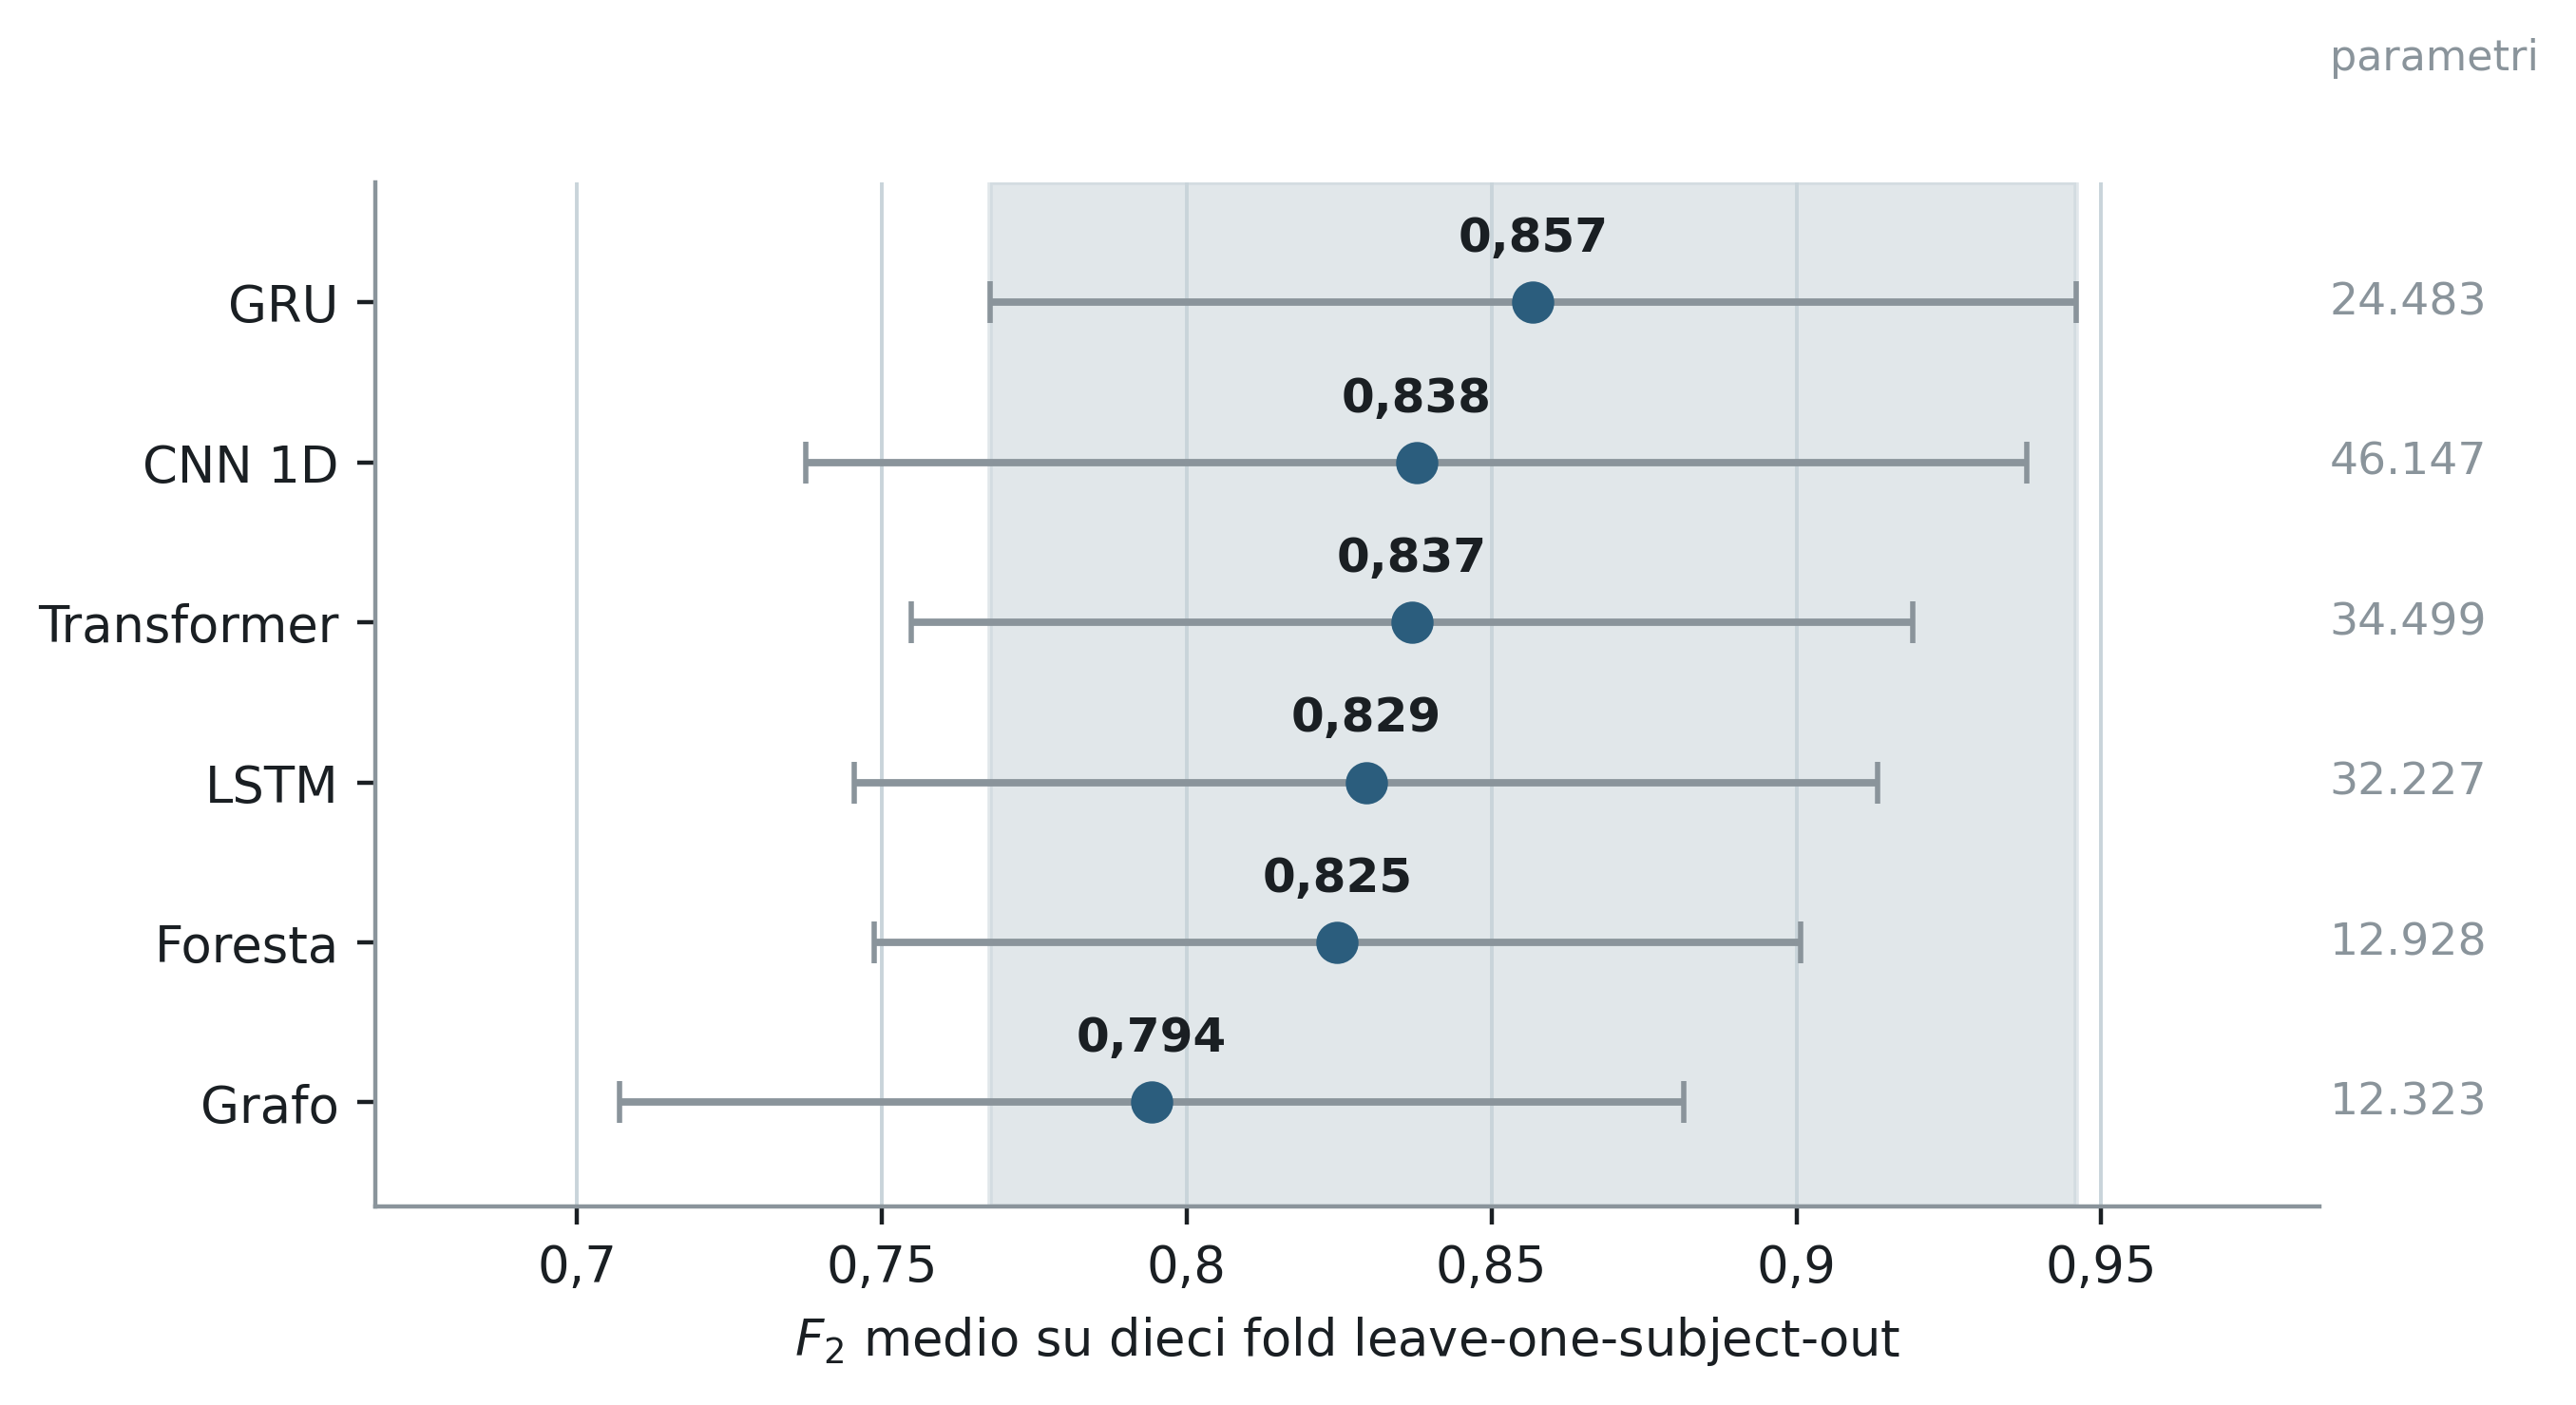
\includegraphics[width=.86\textwidth]{figure/fig_architetture.png}
\caption{Confronto fra le sei architetture a parità di rappresentazione e
protocollo. Le barre di errore rappresentano la \textbf{deviazione standard}
calcolata sui dieci fold della validazione LOSO.}
\label{fig:architetture}
\end{figure}

Il numero di parametri addestrabili non mostra una relazione evidente con le prestazioni. La CNN 1D è il modello neurale con il maggior numero di parametri ma non raggiunge il valore maggiore di $F_2$, mentre la GRU utilizza circa il 24\% di parametri in meno rispetto alla LSTM ottenendo una prestazione superiore.

Il confronto appaiato fold per fold conferma questa lettura. Rispetto alla GRU si ottengono $t=+0{,}59$ per la CNN, $t=-0{,}43$ per la Random Forest, $t=-0{,}82$ per il Transformer e $t=-1{,}20$ per la LSTM.

La rete a grafo raggiunge invece $t=-3{,}00$, oltre il valore critico non corretto di 2,31. Il segno è però negativo, quindi la differenza corrisponde a una prestazione inferiore rispetto alla GRU. Inoltre vengono effettuati cinque confronti contro lo stesso riferimento: applicando una correzione per confronti multipli, il valore critico aumenta e la differenza non rimane significativa.

I risultati non forniscono quindi evidenza che una delle architetture considerate superi la GRU. Più in generale, con il protocollo adottato e con dieci soggetti \textbf{non emerge un'evidenza sufficientemente forte da attribuire alla scelta dell'architettura un ruolo dominante nel determinare la prestazione}: gli scarti fra modelli rimangono dello stesso ordine, o inferiori, alla variabilità osservata fra soggetti. La Random Forest impiegata nel sistema finale non viene quindi giustificata come il modello migliore in assoluto, ma come la scelta ingegneristicamente più conveniente nel compromesso fra prestazione, semplicità, costo di addestramento e requisiti di \emph{deployment}, come discusso nel Capitolo~\ref{cap:edge}.

\paragraph{Quanto vale l'ordine delle colonne.}

Una verifica successiva permette di dare una misura concreta a questa cautela. La foresta casuale è stata riaddestrata due volte sulle \emph{stesse} dodici grandezze, con gli stessi dati, lo stesso protocollo e lo stesso seme, cambiando soltanto \textbf{l'ordine in cui due colonne adiacenti compaiono nell'elenco} --- l'ottava e la nona, che il criterio di selezione ordina in modo pressoché equivalente.

\begin{table}[ht]
\centering
\caption{Effetto del solo ordine delle colonne sulla foresta casuale. Stesse
grandezze, stessi dati, stesso seme: cambia soltanto la posizione reciproca
di due colonne adiacenti nell'elenco.}
\label{tab:ordine}
\begin{tabular}{lcccc}
\toprule
\textbf{Ordine} & \textbf{$F_2$} & \textbf{Recall} & \textbf{FN} & \textbf{FP} \\
\midrule
Elenco originale & $0{,}808 \pm 0{,}103$ & 0,835 & 248 & 499 \\
Ottava e nona scambiate & $0{,}819 \pm 0{,}100$ & 0,842 & 239 & 445 \\
\bottomrule
\end{tabular}
\end{table}

La differenza è di \textbf{0,011} di $F_2$. Il valore va confrontato con la Tabella~\ref{tab:numerosita}: la differenza fra GRU e Random Forest, che quella analisi stima richiedere oltre quattrocento soggetti per essere dichiarata, vale $0{,}012$. \emph{Una differenza che il capitolo discute come confronto fra modelli è quindi della stessa grandezza dell'ordine, arbitrario, in cui le colonne vengono elencate.} L'osservazione non invalida i confronti precedenti, che sono condotti a parità di ordine; fissa però una scala sotto la quale nessuna differenza fra configurazioni può essere interpretata.

\subsection{Analisi delle differenze e numerosità campionaria}
\label{sec:numerosita}

La forte dispersione osservata nei confronti precedenti rende utile stimare quanti soggetti sarebbero necessari per distinguere alcune delle differenze misurate. Poiché le configurazioni vengono valutate sugli stessi soggetti, l'analisi può essere effettuata in forma appaiata.

La Tabella~\ref{tab:numerosita} riporta, per alcuni confronti rappresentativi, la differenza osservata, il valore del test appaiato e una stima della numerosità necessaria per rilevare l'effetto con potenza pari all'80\%.

\begin{table}[ht]
\centering
\caption{Numerosità stimata per rilevare alcune delle differenze osservate con
potenza dell'80\%.}
\label{tab:numerosita}
\begin{tabular}{lccc}
\toprule
\textbf{Confronto} & \textbf{Differenza} &
\textbf{$t$} & \textbf{Soggetti necessari} \\
\midrule
Definizione del compito & $-0{,}309$ & $-6{,}85$ & 2 \\
GRU vs grafo & $-0{,}119$ & $-3{,}00$ & 11 \\
Effetto delle grandezze integrali & $-0{,}022$ & $-1{,}53$ & 34 \\
Finestra 22 vs 44 & $+0{,}033$ & $+1{,}23$ & 52 \\
GRU vs LSTM & $-0{,}036$ & $-1{,}20$ & 57 \\
GRU vs Random Forest & $-0{,}012$ & $-0{,}43$ & 436 \\
\bottomrule
\end{tabular}
\end{table}

Il confronto fra GRU e Random Forest è quello più indicativo: uno scarto medio di $0{,}012$ richiederebbe oltre quattrocento soggetti per poter essere rilevato con la potenza considerata, ed è esattamente la grandezza che la Tabella~\ref{tab:ordine} attribuisce al solo ordine delle colonne. UP-Fall contiene complessivamente 17 partecipanti, dei quali dieci vengono utilizzati nella presente analisi.

Al contrario, alcune modifiche nella definizione del compito producono differenze molto maggiori e risultano osservabili già con un numero ridotto di soggetti. Questo suggerisce che, nella scala del problema considerato, alcune scelte metodologiche incidano molto più della scelta fra architetture con capacità simile.

Le architetture non sono state sottoposte a una ricerca sistematica degli iperparametri. I risultati devono quindi essere interpretati come un confronto fra le configurazioni effettivamente utilizzate e non come una classifica generale delle rispettive famiglie di modelli.

\section{Analisi di sensibilità}

Oltre alle scelte principali, sono stati verificati alcuni parametri che potrebbero influenzare il comportamento del sistema: la dimensione della Random Forest, la frequenza di campionamento, la lunghezza della finestra temporale, la disponibilità dei landmark e il rumore presente nelle coordinate.

Queste verifiche non hanno lo scopo di individuare un valore ottimo per ogni parametro, ma di controllare se le conclusioni precedenti dipendano fortemente da una singola scelta della pipeline.

\subsection{Dimensione del modello}
\label{sec:dimensione}

La prima analisi riguarda la dimensione della Random Forest. La configurazione utilizzata nel sistema impiega 50 alberi, ma questo valore era stato inizialmente ereditato dal prototipo e non scelto sulla base di un confronto sperimentale. Sono state quindi considerate sei dimensioni comprese fra 10 e 400 alberi, mantenendo invariati dati, feature e protocollo di valutazione.

La Figura~\ref{fig:dimensione} riporta, per ciascuna configurazione, il valore medio di $F_2$ e il tempo necessario per classificare una finestra.

\begin{figure}[ht]
    \centering
    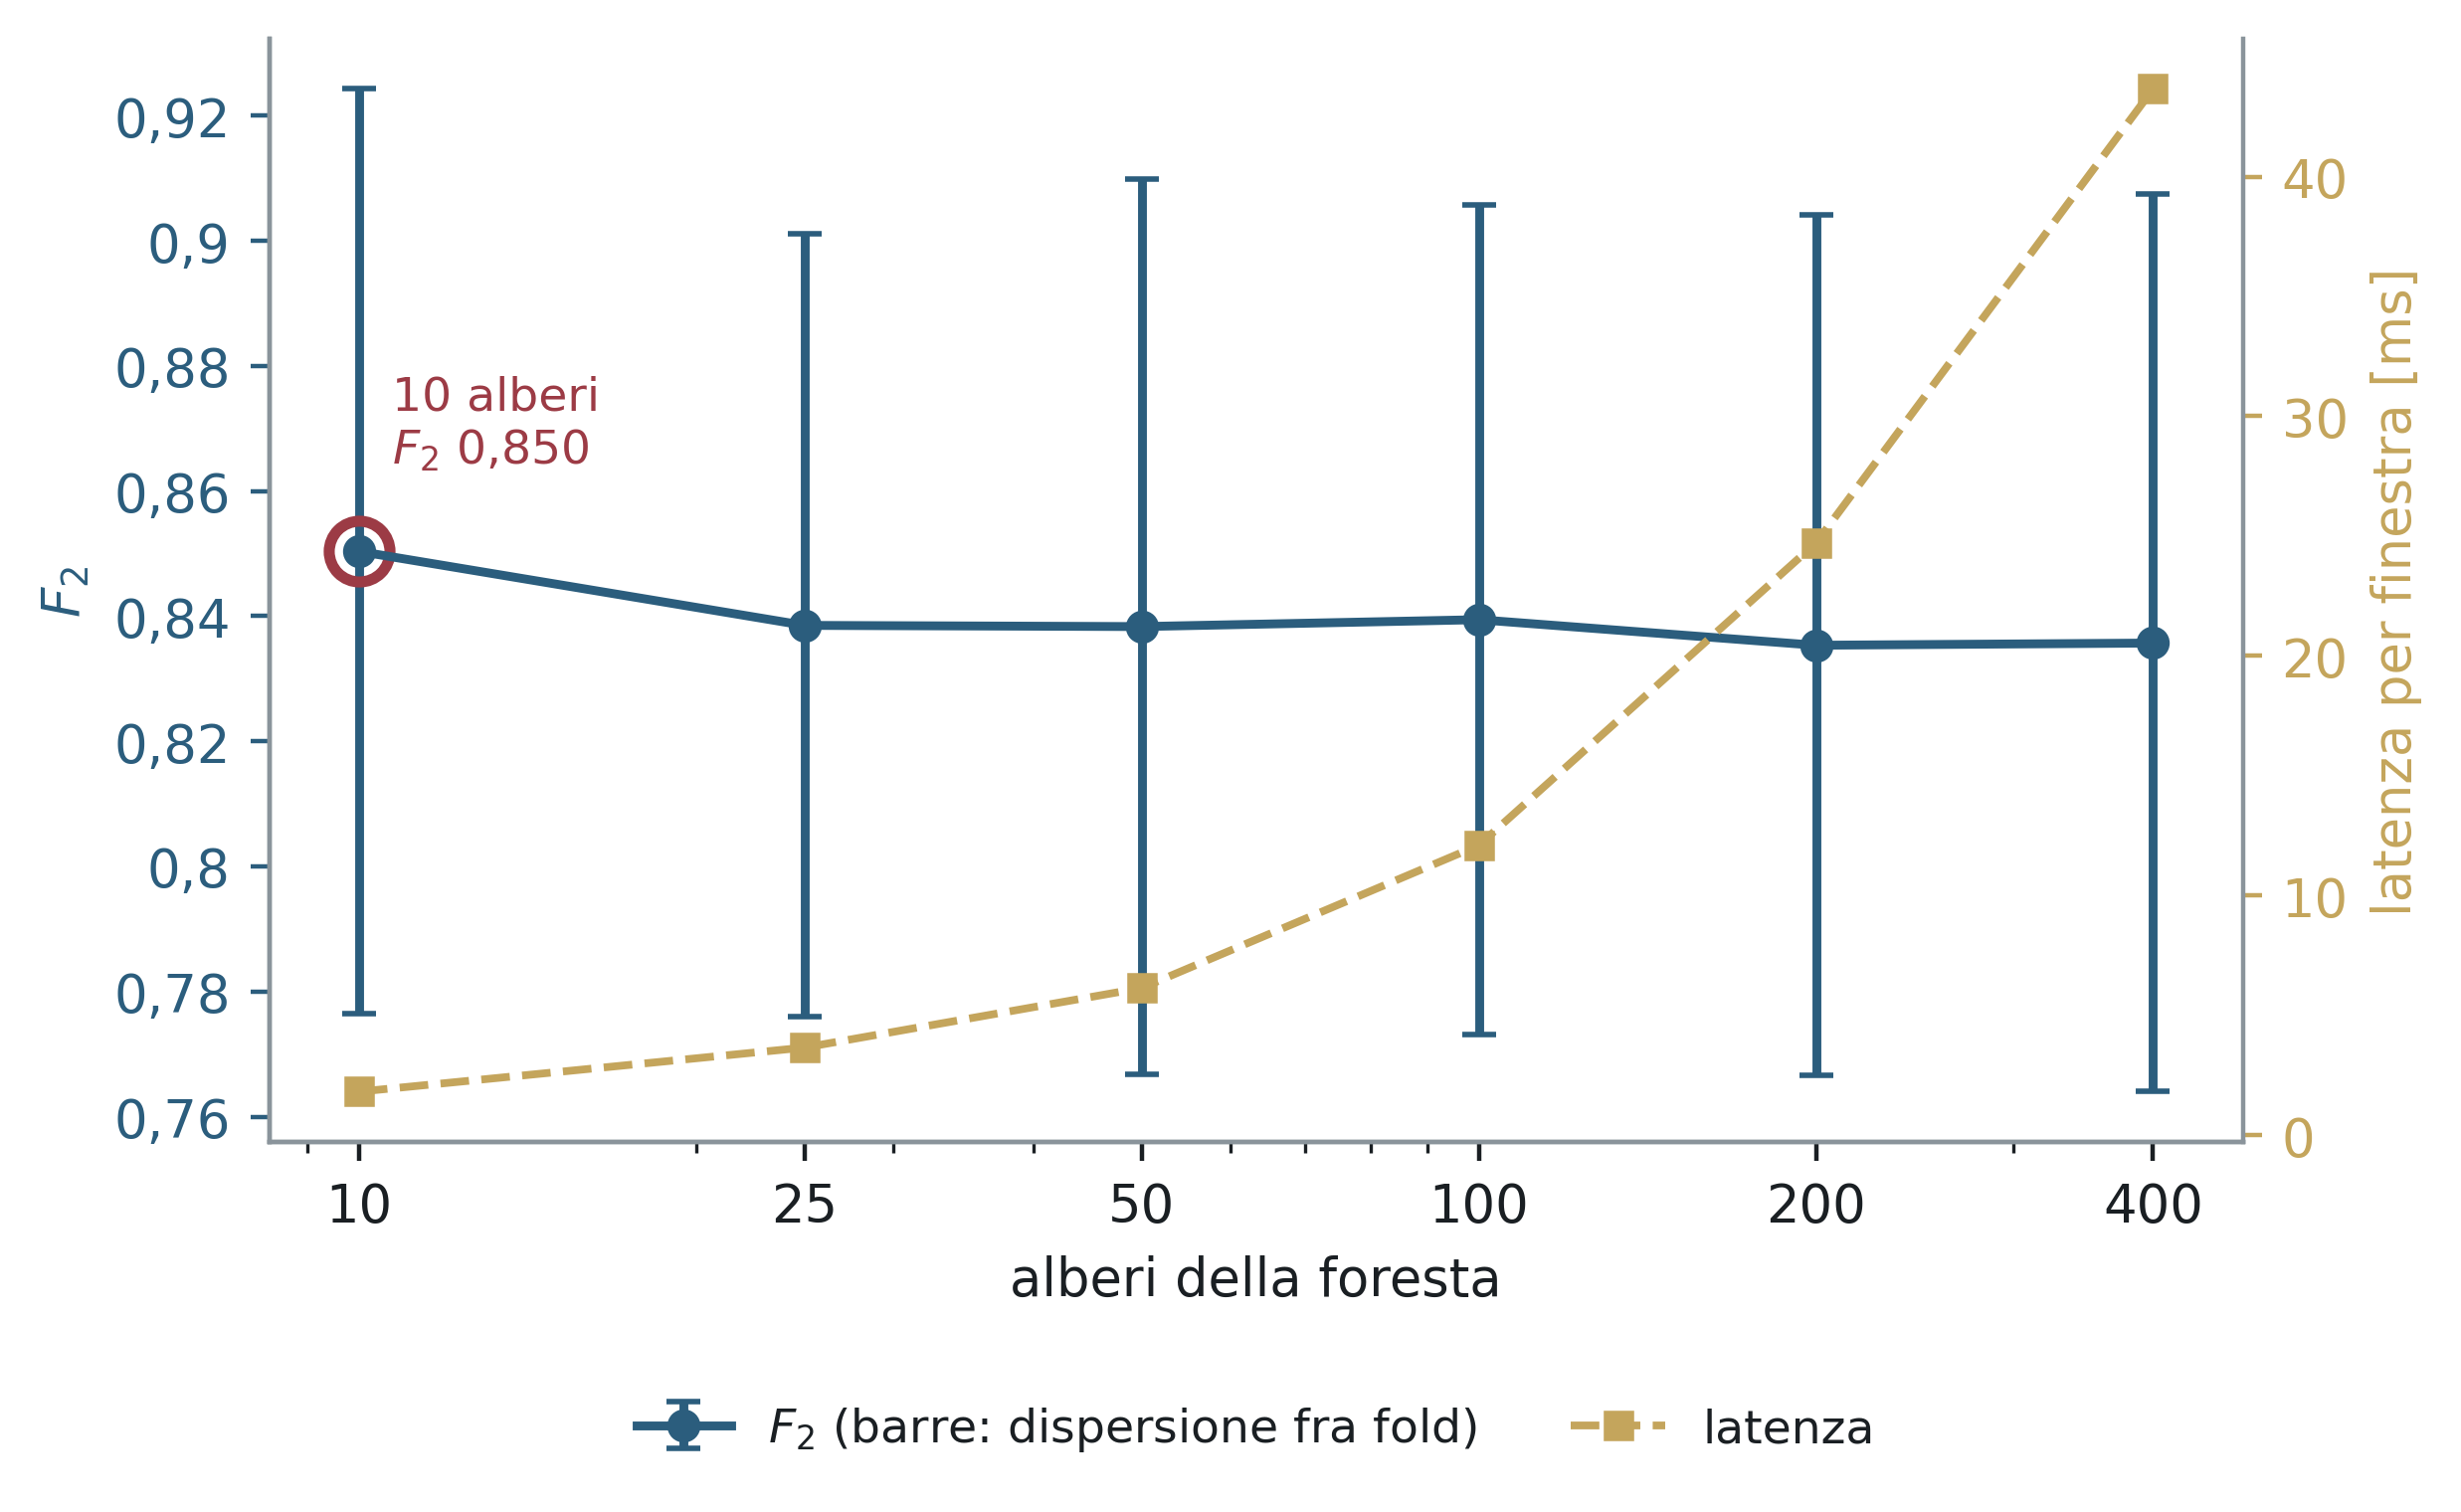
\includegraphics[width=.82\textwidth]{figure/fig_dimensione.png}
    \caption{Prestazioni e latenza al variare del numero di alberi della
    Random Forest. Le barre di errore rappresentano la deviazione standard fra
    i soggetti. La misura è stata effettuata nell'impianto a cinque soggetti e
    i tempi sono misurati sul calcolatore di sviluppo.}
    \label{fig:dimensione}
\end{figure}

Con 50 alberi si ottiene un $F_2$ pari a 0,906 e una latenza di 4,47~ms per finestra. Aumentando il numero di alberi a 200, il valore di $F_2$ è pari a 0,888, mentre la latenza sale a 17,98~ms. Anche per le altre dimensioni considerate non emerge un miglioramento regolare delle prestazioni, mentre il costo computazionale cresce all'aumentare del numero di alberi.

\emph{I tempi riportati in questa sezione sono misurati sul calcolatore di sviluppo e non sul dispositivo edge.} Sulla piattaforma di destinazione lo stesso classificatore costa circa un ordine di grandezza in più, come riportato nel Capitolo~\ref{cap:edge}; il confronto fra le sei dimensioni resta valido perché tutte sono misurate nelle stesse condizioni, ma il valore assoluto non descrive il sistema installato.

Le barre di dispersione delle diverse configurazioni risultano inoltre ampiamente sovrapposte. Non è quindi possibile affermare che 50 alberi costituiscano il valore ottimo in termini di accuratezza. Il risultato mostra piuttosto che, nell'intervallo analizzato, aumentare la dimensione della foresta non produce un beneficio misurabile e comporta invece un aumento del tempo di inferenza.

Per questo motivo la configurazione a 50 alberi viene mantenuta nelle prove successive. I valori di questa analisi provengono dall'impianto sperimentale a cinque soggetti e devono quindi essere considerati soprattutto per descrivere l'andamento rispetto alla dimensione del modello.

\subsection{Effetto del frame rate}
\label{sec:framerate}

Un secondo parametro rilevante è la frequenza con cui vengono elaborati i fotogrammi. UP-Fall è acquisito a circa 18~fps, mentre l'esecuzione su un dispositivo con risorse limitate può richiedere una frequenza inferiore. È stato quindi verificato l'effetto del dimezzamento del frame rate da 18 a 9~fps.

\begin{table}[ht]
\centering
\caption{Effetto del dimezzamento del frame rate sulle prestazioni. La misura
proviene dall'impianto sperimentale a cinque soggetti.}
\label{tab:framerate}
\begin{tabular}{lcc}
\toprule
 & \textbf{18 fps} & \textbf{9 fps} \\
\midrule
Cadute non rilevate & 6,8\% & 12,4\% \\
Variazione di $F_2$ & -- & $-0{,}045$ \\
\bottomrule
\end{tabular}
\end{table}

La variazione complessiva di $F_2$ è pari a circa $-0{,}045$ e rimane quindi dello stesso ordine della dispersione osservata fra soggetti. Il dato cambia però se vengono considerati separatamente i falsi negativi: la quota di cadute non rilevate passa dal 6,8\% al 12,4\%.

Il dimezzamento della frequenza comporta quindi una perdita soprattutto in termini di recall. La variazione di $F_2$ appare più contenuta perché il peggioramento della recall viene in parte compensato da una variazione della precision. Questo risultato conferma l'importanza di considerare separatamente i diversi tipi di errore e non soltanto una metrica aggregata.

La frequenza di 9~fps rimane comunque di interesse per il sistema finale, poiché rappresenta una condizione compatibile con le prestazioni ottenibili sul dispositivo edge. Il confronto con l'hardware verrà ripreso nel Capitolo~\ref{cap:edge}.

\subsection{Sensibilità alla perdita di landmark}
\label{sec:occlusioni}

La disponibilità dei landmark può ridursi quando alcune parti del corpo non sono correttamente osservate dallo stimatore di posa. Per verificare quanto il classificatore sia sensibile alla perdita di alcuni landmark è stata effettuata una simulazione controllata. Il punto considerato non disponibile viene mantenuto all'ultima posizione osservata, invece di essere posto a zero. In questo modo si evita di introdurre artificialmente uno spostamento verso l'origine dell'immagine e si riproduce una condizione simile alla propagazione temporale utilizzata da uno stimatore di posa.

Sono stati mascherati sia gruppi anatomici sia gruppi casuali di dimensione crescente. La prestazione di riferimento senza alcun mascheramento è $F_2=0{,}853\pm0{,}071$.

\begin{table}[ht]
\centering
\caption{Variazione di $F_2$ ottenuta congelando diversi gruppi di landmark
all'ultima posizione osservata.}
\label{tab:occlusioni}
\begin{tabular}{lcc}
\toprule
\textbf{Gruppo} & \textbf{Punti} & \textbf{$\Delta F_2$} \\
\midrule
Spalle & 2 & $-0{,}037$ \\
Caviglie & 2 & $-0{,}012$ \\
Metà sinistra & 6 & $-0{,}004$ \\
Naso & 1 & $-0{,}002$ \\
Ginocchia + caviglie & 4 & $+0{,}001$ \\
Anche & 2 & $+0{,}015$ \\
\midrule
Casuale 11\% & 1 & $-0{,}002$ \\
Casuale 22\% & 2 & $+0{,}001$ \\
Casuale 33\% & 3 & $+0{,}003$ \\
Casuale 55\% & 5 & $-0{,}032$ \\
\bottomrule
\end{tabular}
\end{table}

\begin{figure}[ht]
\centering
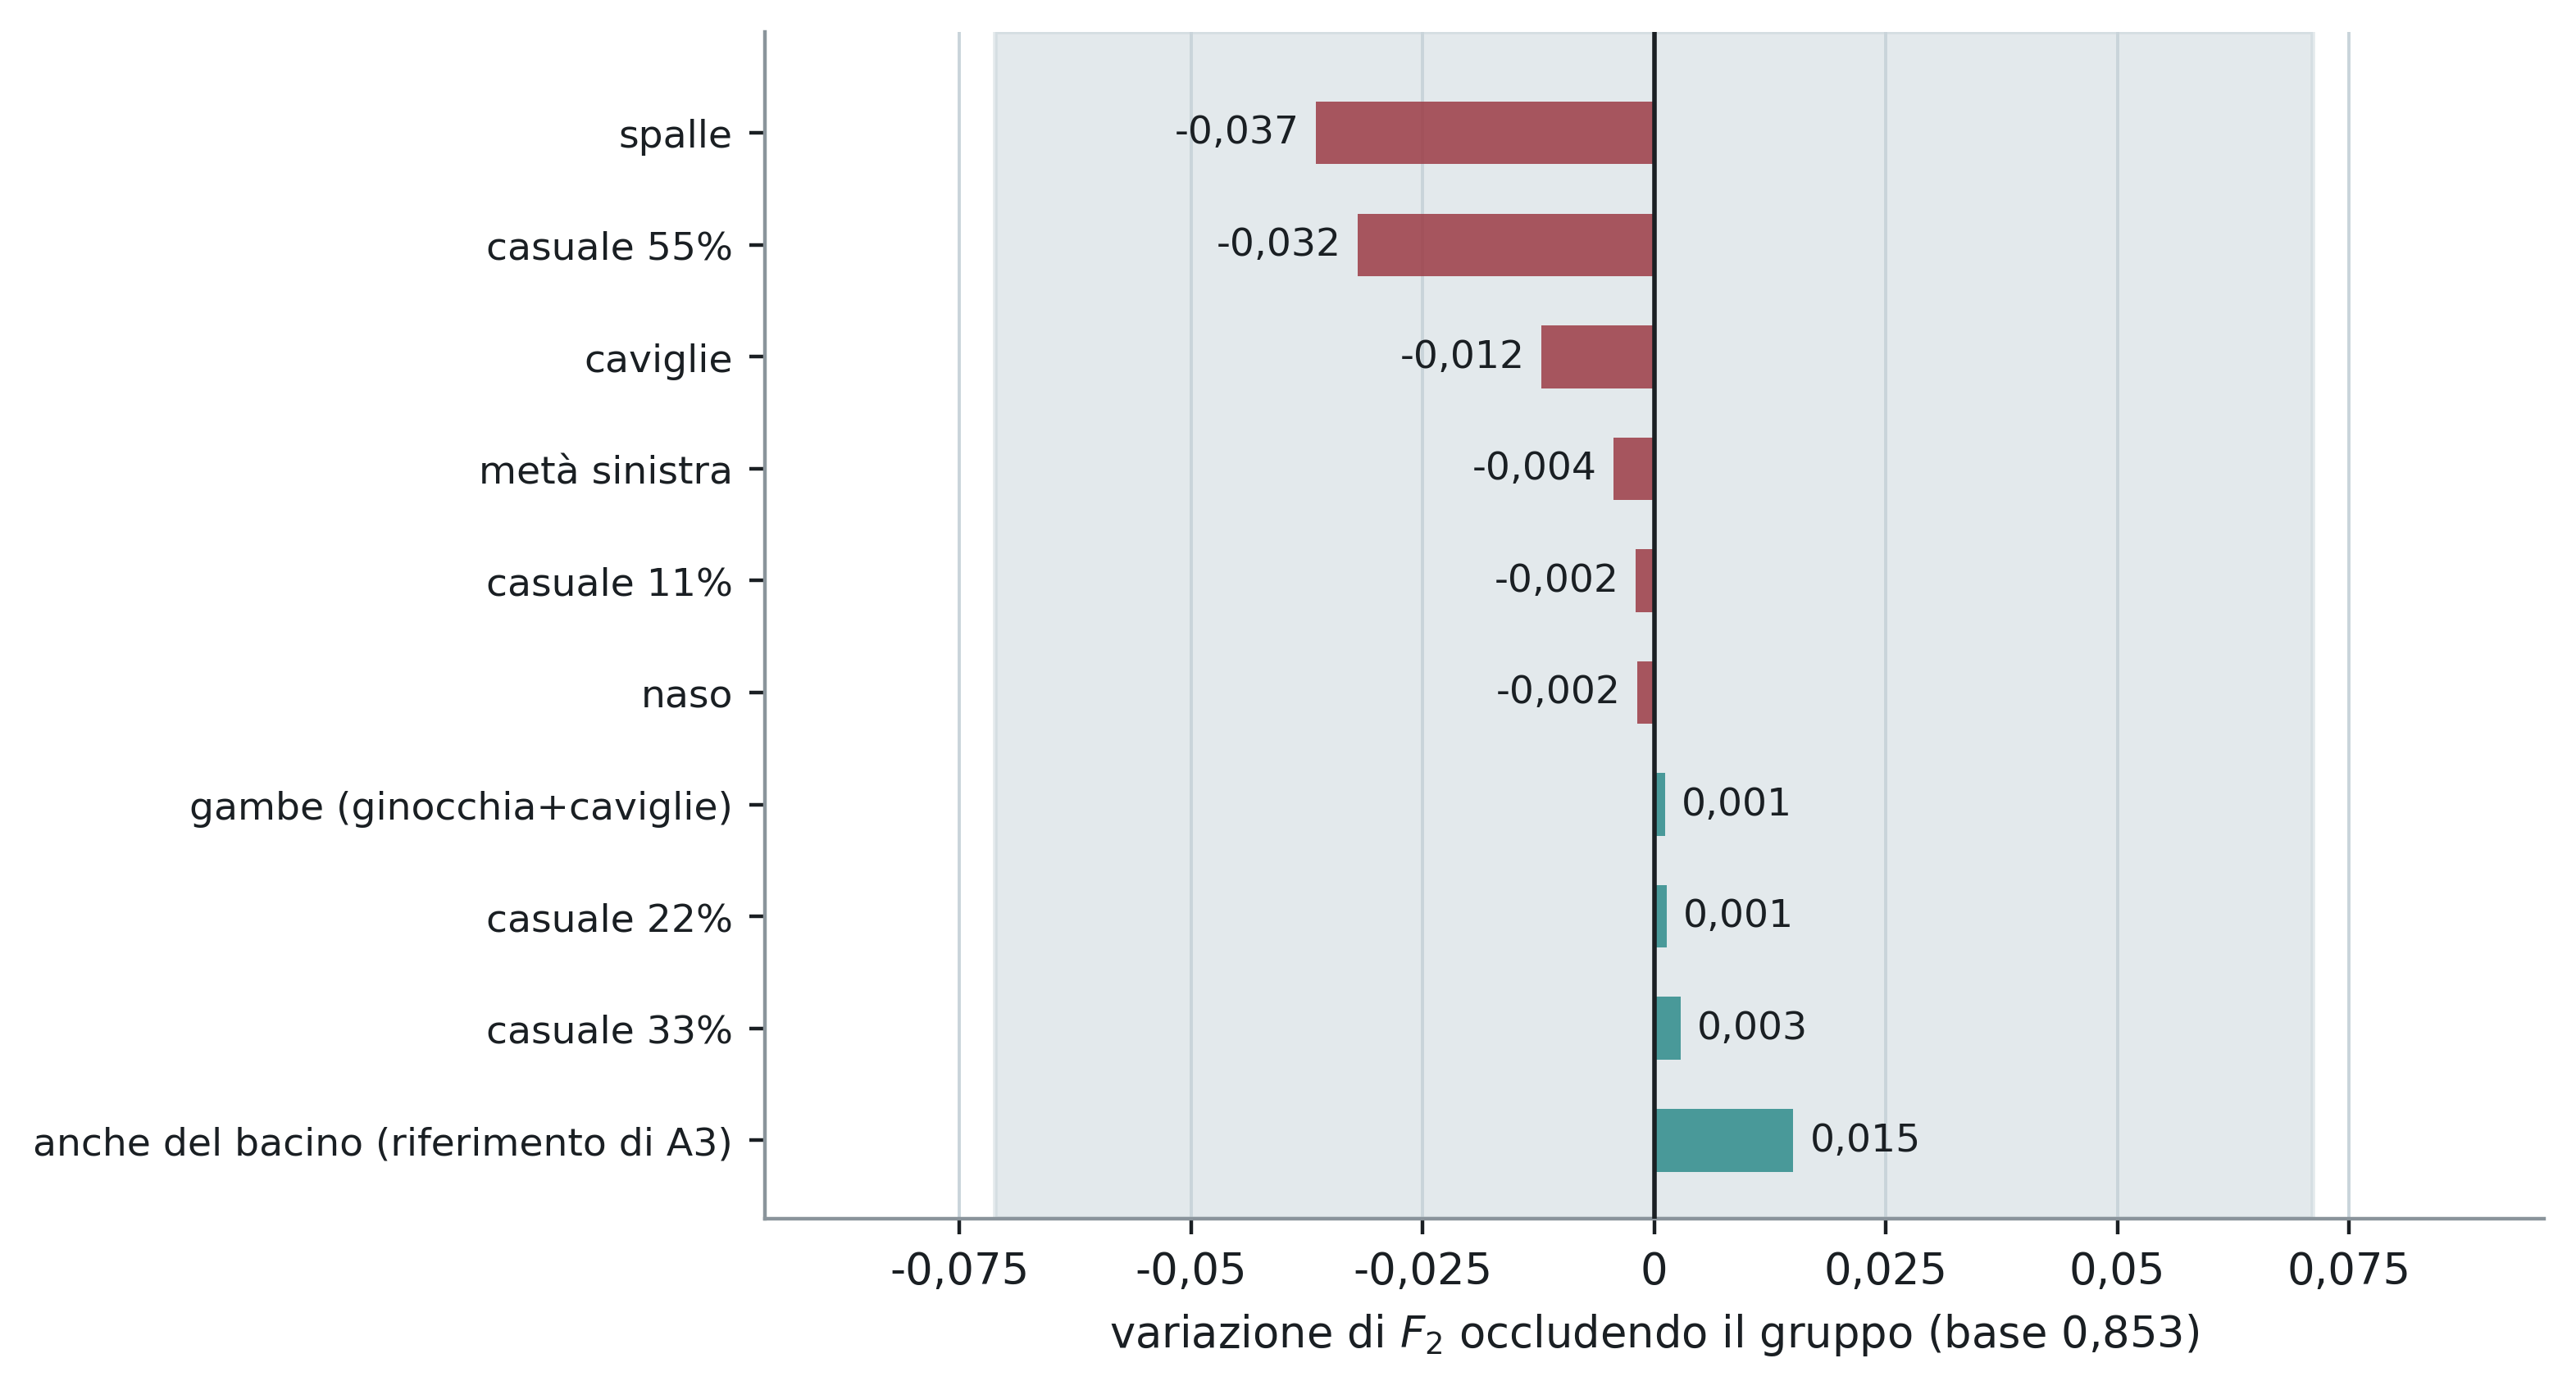
\includegraphics[width=.86\textwidth]{figure/fig_occlusioni.png}
\caption{Effetto del mascheramento simulato dei diversi gruppi di landmark.
La banda rappresenta la deviazione standard fra soggetti della configurazione
di riferimento, cioè senza alcun mascheramento.}
\label{fig:occlusioni}
\end{figure}

Il peggioramento massimo è pari a 0,037 di $F_2$, quindi circa due volte inferiore alla dispersione fra soggetti. La conclusione che i dati sostengono è quindi la seguente: \textbf{nella simulazione controllata non emerge un singolo gruppo di landmark la cui perdita determini da sola il collasso del sistema}. Le variazioni positive di $+0{,}001$ e $+0{,}003$ osservate per alcuni gruppi non vanno lette come miglioramenti, ma come fluttuazioni sperimentali di ampiezza confrontabile con l'incertezza della misura.

Le spalle sono l'unico gruppo anatomico che costi più di un gruppo casuale della stessa dimensione. Rifacendo la misura con il sottoinsieme di grandezze precedente, però, le spalle tornano a $-0{,}019$: la sensibilità non dipende dai punti del corpo ma da quali dodici grandezze il criterio di selezione ha scelto. Fra i due sottoinsiemi cambia una colonna --- entra l'angolo del tronco, che è il vettore fra spalle e anche --- e con essa si sposta il punto su cui il sistema è vulnerabile. Non è quindi che l'informazione sia distribuita in sé: lo è per un dato insieme di grandezze.

Il risultato va interpretato come una verifica di perturbazioni controllate dei landmark. Congelare un punto all'ultima posizione disponibile è un esperimento utile, ma non riproduce completamente il comportamento di uno stimatore di posa in presenza di un'occlusione reale, ad esempio dovuta a mobili od oggetti che nascondono una parte consistente del corpo.

È stata infine verificata la sensibilità al rumore delle coordinate aggiungendo una perturbazione gaussiana indipendente ai landmark. La deviazione standard $\sigma$ viene espressa come frazione della lunghezza del torso, in modo da rendere l'intensità della perturbazione indipendente dalla scala apparente della persona.

Sono stati confrontati il set senza grandezze integrali, quello che include le grandezze integrali e il sottoinsieme selezionato tramite DTW. Anche al livello massimo considerato, $\sigma=0{,}04$, il peggioramento maggiore è pari a 0,031 di $F_2$, quindi ancora inferiore alla dispersione fra soggetti.

Il risultato non implica che le grandezze integrali eliminino il rumore. Percorso, escursione e discesa possono infatti aumentare in presenza di perturbazioni. La verifica mostra soltanto che, per il rumore indipendente e per le intensità considerate, l'effetto sulle prestazioni finali rimane limitato.

\section{Effetto della definizione del compito}
\label{sec:compito-risultati}

Le analisi precedenti modificano il modo in cui uno stesso problema viene rappresentato o classificato. Un'ulteriore scelta riguarda invece la definizione stessa della classe positiva.

Come discusso nel Capitolo~\ref{cap:metodologia}, una caduta comprende almeno due condizioni differenti: la transizione dinamica con cui la persona perde l'equilibrio e lo stato successivo nel quale il soggetto rimane a terra. Queste due condizioni possono essere trattate come un'unica classe oppure separate.

Sono stati quindi confrontati tre compiti mantenendo invariati modello, feature e protocollo:

\begin{itemize}
    \item \textbf{evento}: è positiva soltanto la transizione di caduta;
    \item \textbf{stato}: è positiva la condizione successiva, con il soggetto
          già a terra;
    \item \textbf{allarme}: vengono considerate positive entrambe le
          condizioni.
\end{itemize}

Una particolare attenzione viene posta alle attività in cui una persona si sdraia volontariamente. Queste finestre rappresentano negativi difficili, perché la configurazione finale del corpo può essere molto simile a quella di una persona rimasta a terra dopo una caduta.

\begin{table}[ht]
\centering
\caption{Prestazioni ottenute con le tre definizioni del compito a parità di
modello, feature e protocollo. L'ultima colonna riporta la quota di finestre
segnalate come positive durante l'azione di sdraiarsi volontariamente.}
\label{tab:compiti}
\begin{tabular}{lcccc}
\toprule
\textbf{Compito} & \textbf{Prevalenza} & \textbf{$F_2$} &
\textbf{Precision} & \textbf{Negativi difficili} \\
\midrule
Evento & 0,047 & $0{,}831\pm0{,}072$ & 0,924 & 0,0\% \\
Stato & 0,089 & $0{,}704\pm0{,}084$ & 0,755 & 12,5\% \\
Allarme & 0,115 & $0{,}810\pm0{,}068$ & 0,833 & 13,1\% \\
\bottomrule
\end{tabular}
\end{table}

\begin{figure}[ht]
\centering
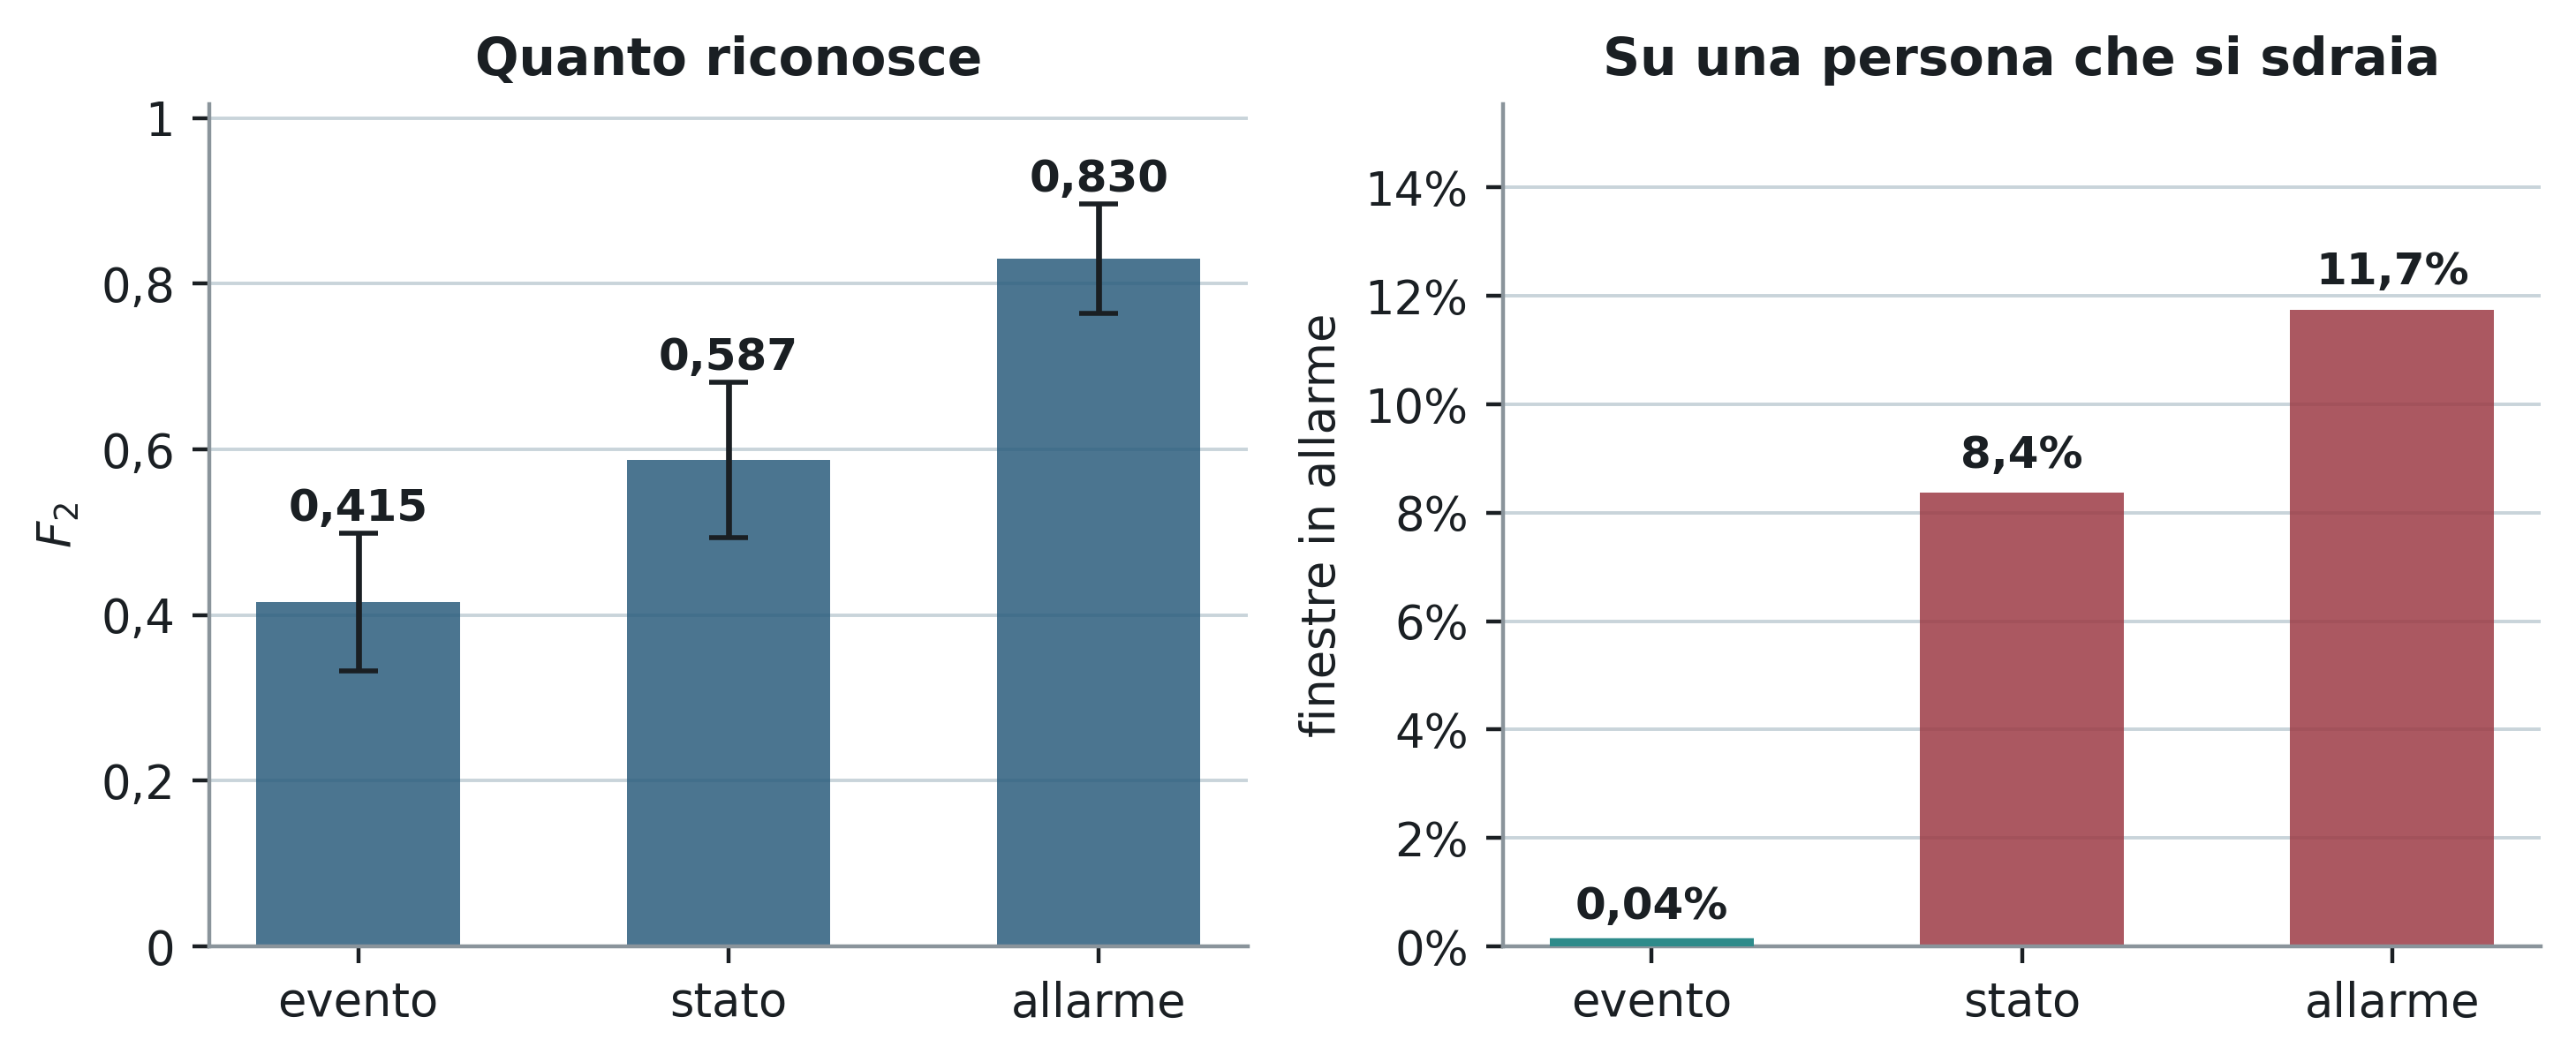
\includegraphics[width=.92\textwidth]{figure/fig_compiti.png}
\caption{Confronto fra le tre definizioni del compito. A sinistra è riportato
l'$F_2$, con barre di errore pari alla deviazione standard fra i dieci
soggetti; a destra è mostrata la quota di finestre segnalate come positive
durante l'azione di sdraiarsi volontariamente.}
\label{fig:compiti}
\end{figure}

Il compito evento raggiunge il valore più elevato di $F_2$, pari a 0,831, e la precision più alta, pari a 0,924. Il risultato più importante riguarda però i negativi difficili: nessuna delle 2234 finestre corrispondenti a persone sdraiate volontariamente viene classificata come positiva.

Il compito stato produce invece falsi allarmi sul 12,5\% di queste finestre, mentre il compito allarme raggiunge il 13,1\%.

La differenza deriva dalla natura dell'informazione richiesta. Quando il classificatore deve riconoscere lo stato finale, una persona distesa dopo una caduta e una persona che si è sdraiata volontariamente possono presentare una geometria molto simile. Nel compito evento, invece, ciò che viene ricercato è la transizione che conduce a quella configurazione e non la configurazione stessa.

La definizione della classe positiva ha quindi un effetto maggiore di quello osservato nel confronto fra le architetture. Questo risultato motiva la scelta di considerare la caduta principalmente come un evento dinamico e non come il semplice riconoscimento di una persona a terra.

\section{Trasferimento a un dataset esterno}
\label{sec:domainshift}

La validazione LOSO permette di verificare il comportamento su persone non osservate durante l'addestramento, ma tutte le registrazioni provengono comunque dallo stesso dataset. Camera, ambiente, procedura di acquisizione e annotazioni rimangono quindi sostanzialmente gli stessi.

Per verificare un livello di trasferimento più severo, il sistema viene applicato a UR-Fall, un dataset acquisito indipendentemente da UP-Fall e caratterizzato da soggetti, ambienti e condizioni di ripresa differenti.

Prima del confronto è stato necessario rendere coerente la semantica delle annotazioni. UP-Fall distingue le fasi temporali dell'evento, mentre le annotazioni originali di UR-Fall descrivono principalmente la postura del soggetto. In particolare, la condizione di persona distesa non può essere automaticamente interpretata come una caduta in corso.

UR-Fall è stato quindi riestratto utilizzando lo stesso motore geometrico impiegato per UP-Fall e le annotazioni sono state riportate alle tre fasi utilizzate nel presente lavoro. L'estrazione produce 11400 fotogrammi distribuiti su 67 registrazioni e tutte le 33 grandezze previste dalla pipeline.

La posa risulta valida nell'81,0\% dei fotogrammi, contro il 95,9\% ottenuto su UP-Fall considerando entrambe le telecamere. Il dato indica già una differenza significativa nelle condizioni di acquisizione e rende il trasferimento più severo rispetto alla sola variazione del soggetto all'interno dello stesso dataset.

Il confronto viene effettuato senza utilizzare UR-Fall per addestrare il classificatore. Il modello viene quindi addestrato sui dati di UP-Fall e applicato direttamente al nuovo archivio.

\subsection{Metriche indipendenti dalla soglia}
\label{sec:prauc}

La diversa prevalenza delle classi rende poco informativo confrontare direttamente un singolo valore di $F_2$ ottenuto nei due dataset. La precision, e quindi anche l'$F_2$, dipende infatti dalla quota di esempi positivi presenti nell'insieme considerato.

Per valutare se il classificatore mantiene la capacità di ordinare le finestre positive prima di applicare una soglia viene quindi considerata l'area sotto la curva precision--recall, o PR-AUC.

Per un classificatore casuale la PR-AUC attesa coincide con la prevalenza della classe positiva. Il rapporto
\[
G_{\mathrm{PR}}
=
\frac{\mathrm{PR\text{-}AUC}}
     {\mathrm{prevalenza}}
\]

può quindi essere interpretato come il guadagno rispetto a una classificazione casuale nello stesso dataset.

La Tabella~\ref{tab:esterno} riporta il risultato su UR-Fall per le configurazioni considerate.

\begin{table}[ht]
\centering
\caption{Trasferimento da UP-Fall a UR-Fall. Il guadagno è ottenuto
rapportando la PR-AUC alla prevalenza del dataset di destinazione. L'ultima
colonna riporta l'$F_2$ alla soglia fissata nel dominio di addestramento e non
ricalibrata su quello di destinazione.}
\label{tab:esterno}
\begin{tabular}{lccc}
\toprule
\textbf{Configurazione} & \textbf{PR-AUC} &
\textbf{Guadagno} & \textbf{$F_2$ a $\theta=0{,}50$} \\
\midrule
Configurazione schierata precedente & 0,169 & 1,8$\times$ & 0,034 \\
A3 senza integrali & 0,440 & 3,4$\times$ & 0,404 \\
A3 con integrali & 0,466 & 3,6$\times$ & 0,479 \\
Sottoinsieme DTW & 0,660 & 5,1$\times$ & 0,630 \\
\bottomrule
\end{tabular}
\end{table}

\begin{figure}[ht]
\centering
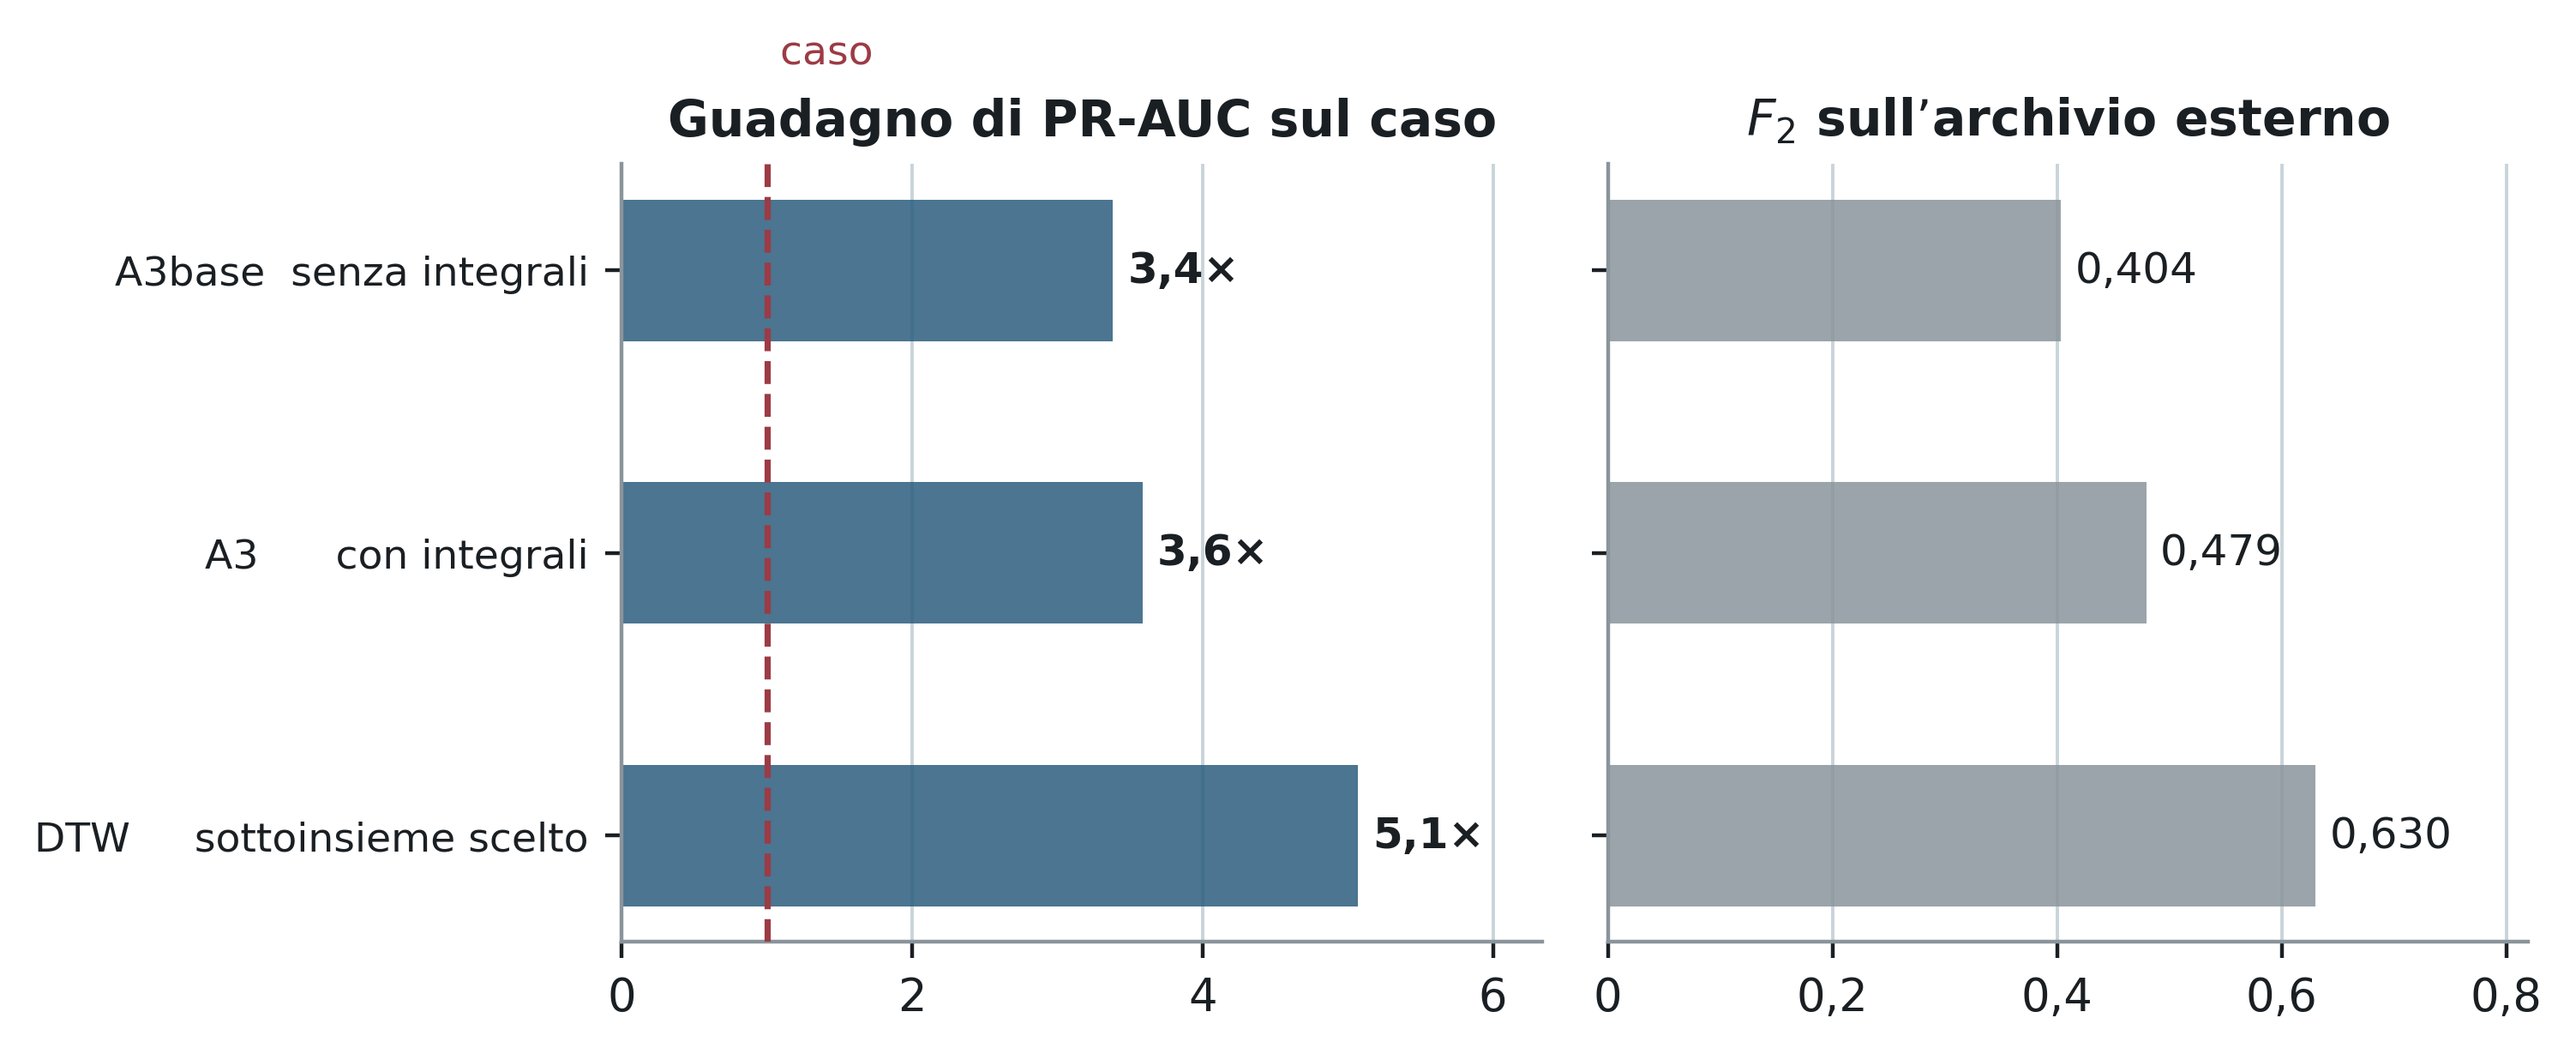
\includegraphics[width=.86\textwidth]{figure/fig_esterno.png}
\caption{Prestazioni nel trasferimento a UR-Fall. A sinistra è mostrato il
guadagno della PR-AUC rispetto al caso, mentre a destra è riportato l'$F_2$
alla soglia fissata nel dominio di addestramento.}
\label{fig:esterno}
\end{figure}

Il sottoinsieme selezionato tramite DTW raggiunge una PR-AUC pari a 0,660, corrispondente a circa 5,1 volte la prestazione attesa dal caso. Il valore è nettamente superiore a quello della configurazione precedente, che raggiungeva soltanto 1,8 volte il caso.

Anche l'introduzione delle grandezze integrali produce un miglioramento, da 3,4 a 3,6 volte il caso, ma il salto principale è associato alla rappresentazione complessiva corretta e al sottoinsieme finale di feature.

Il risultato mostra che una parte dell'informazione appresa su UP-Fall sopravvive al passaggio a UR-Fall. Allo stesso tempo, la riduzione rispetto alle prestazioni ottenute nel dominio di addestramento indica che il trasferimento non è completo. Una PR-AUC superiore alla prevalenza significa infatti che il modello conserva capacità discriminativa, ma non che tale capacità rimanga invariata.

\subsection{Calibrazione e capacità discriminativa}
\label{sec:calibrazione}


Il deterioramento osservato su un dataset esterno può derivare da due cause distinte, che la sola PR-AUC non permette di separare. La prima è una perdita di capacità discriminativa: il modello ordina le finestre peggio di quanto facesse nel dominio di addestramento, e un ordinamento che non è più presente non viene recuperato da alcuna scelta della soglia. La seconda è un difetto di calibrazione: l'ordinamento viene conservato, ma i punteggi si collocano su una scala diversa da quella sulla quale la soglia era stata fissata, e la soglia dichiarata non corrisponde più al punto desiderato di quella scala.

La distinzione ha una conseguenza pratica precisa. Una perdita di capacità discriminativa richiede di riaddestrare il modello, mentre un difetto di calibrazione richiede soltanto di ritararne la soglia, con un costo notevolmente inferiore.

Per separare le due componenti viene utilizzata una \emph{soglia oracolo}, ovvero il valore che massimizza l'$F_2$ nel dominio di destinazione utilizzando le etichette di quel dominio. Si tratta di un valore non disponibile in un impiego reale, poiché chi installa il sistema in un'abitazione non dispone di cadute etichettate dell'ambiente di destinazione. La soglia oracolo non rappresenta quindi una prestazione ottenibile, ma un limite superiore che consente di attribuire alla taratura la parte di divario che la taratura potrebbe recuperare.

La misura è ottenuta con lo stesso modello, lo stesso codice e la stessa soglia nei due domini, ed è riportata in \texttt{risultati/campo/pr\_auc\_allineato.json}. Nel dominio di addestramento l'$F_2$ è pari a 0,971 e la PR-AUC a 0,990, corrispondente a 18,7 volte la prevalenza. Su UR-Fall, con la soglia dichiarata $\theta = 0{,}50$, l'$F_2$ scende a 0,034; con la soglia oracolo, pari a 0,118, risale a 0,492.

Dei 0,937 di divario complessivo, 0,457 sono quindi attribuibili alla taratura e 0,480 alla perdita di capacità discriminativa. Le due componenti si dividono il divario quasi esattamente a metà, e il risultato è coerente con la PR-AUC misurata nello stesso insieme, pari a 1,79 volte la prevalenza: il modello continua a ordinare le finestre meglio del caso, ma molto meno bene di quanto facesse nel dominio di addestramento, dove ordinava 18,7 volte meglio.

Questa scomposizione non è in contraddizione con l'$F_2$ pari a 0,630 che la Tabella~\ref{tab:esterno} riporta per il sottoinsieme DTW alla soglia dichiarata, nonostante quel valore risulti superiore allo 0,492 ottenuto con la soglia oracolo. Le due misure riguardano configurazioni diverse e insiemi di finestre diversi: la scomposizione è calcolata sulla configurazione schierata in precedenza, su 1.075 finestre con prevalenza pari al 9,4 per cento, mentre le altre tre righe della tabella provengono da una valutazione distinta, condotta su 884 finestre con prevalenza pari al 13,0 per cento. Per la configurazione attuale la scomposizione fra le due componenti non è stata ricalcolata; il divario di calibrazione è però in quel caso molto minore, dal momento che alla soglia dichiarata l'$F_2$ non subisce un crollo analogo.

Ne discende un'indicazione operativa. Circa metà del divario è recuperabile agendo sulla sola soglia, ma la ricalibrazione richiede etichette che l'ambiente di destinazione non fornisce: la via percorribile è quindi una calibrazione che non utilizzi cadute etichettate, per esempio fissando la soglia su un percentile delle probabilità osservate durante le prime ore di funzionamento ordinario. La parte di divario dovuta alla capacità discriminativa richiede invece di intervenire sull'addestramento, e la direzione indicata dalla Sezione~\ref{sec:viewpoint} è l'utilizzo di una molteplicità di punti di vista.

Il risultato è ottenuto su un solo dataset di destinazione. Con due soli ambienti non è possibile distinguere ciò che è specifico di UR-Fall da ciò che varrebbe per un ambiente nuovo qualunque. La soglia oracolo, inoltre, viene scelta sullo stesso insieme sul quale viene poi misurata, e il valore 0,492 deve essere letto come un limite superiore ottimistico.

% =====================================================================
% LA CODA DI §4.10.2 E' RICOSTRUITA, e queste sono le parole di chi
% ricostruisce, non quelle consegnate. Il testo ricevuto si fermava su
% «Il deterioramento osservato su un dataset esterno puo' derivare da»:
% quella frase e' ripresa alla lettera e continuata. Confrontare con
% l'originale di Overleaf, e tenere quello se dice le stesse cose.
%
% I NUMERI, INVECE, SONO VERIFICATI (2026-09-09) su
% `risultati/campo/pr_auc_allineato.json` e
% `risultati/esterno/urfall_foresta_caduta.json`:
%
%   in dominio    PR-AUC 0,990   18,72x   F2 0,9714
%   UR-Fall       PR-AUC 0,1685   1,79x   F2 0,0345  (soglia 0,50)
%   soglia oracolo 0,1184                 F2 0,4915
%   divario 0,937 = 0,457 taratura + 0,480 capacita' discriminativa
%
% LA CONTRADDIZIONE SEGNALATA IERI NON C'E', ed e' ora dichiarata nel
% testo. Le due misure riguardano configurazioni E POPOLAZIONI diverse:
%
%   - la scomposizione viene da `pr_auc_allineato.json`, che e' la
%     CONFIGURAZIONE SCHIERATA IN PRECEDENZA (A3 a dieci colonne): 1.075
%     finestre, prevalenza 9,4%. E' la prima riga di `tab:esterno`
%     (0,169 / 1,8x / 0,034), e coincide con essa cifra per cifra;
%   - le altre tre righe vengono da `urfall_foresta_caduta.json`: 884
%     finestre, prevalenza 13,0%, modo «caduta». Il sottoinsieme DTW vale
%     0,6597 / 5,07x / F2 0,6304.
%
% Quindi 0,630 e 0,492 non sono confrontabili: configurazione diversa,
% insieme di finestre diverso, prevalenza diversa.
%
% ATTENZIONE, E' UN DIFETTO DELLA TABELLA: `tab:esterno` mette in colonna
% quattro righe di cui la prima e' misurata su una popolazione di finestre
% diversa dalle altre tre. E' ISS-152, aperta il 9 settembre.
%
% RESTA DA FARE, e non e' in questo file:
%   `pipeline/figure_tesi.py:1524` scrive nella figura `fig_dominio` la
%   dicitura «recuperabile ritarando la soglia». Il relatore l'ha letta
%   come «ritirando» e chiede «recuperabile mediante RICALIBRAZIONE della
%   soglia». La figura non compare in QUESTA stesura, che usa
%   `fig:esterno`: la correzione va fatta nello script e la figura
%   rigenerata.
% =====================================================================
